% !BIB TS-program = biber

\RequirePackage[l2tabu,orthodox]{nag}

% TODO: decide if one-sided/two-sided
%\documentclass[headsepline,footsepline,footinclude=false,fontsize=11pt,paper=a4,listof=totoc,bibliography=totoc,BCOR=12mm,DIV=12]{scrbook} % two-sided
\documentclass[headsepline,footsepline,footinclude=false,oneside,fontsize=11pt,paper=a4,listof=totoc,bibliography=totoc]{scrbook} % one-sided

% TODO: change citation style in settings
\PassOptionsToPackage{table,svgnames,dvipsnames}{xcolor}

\usepackage[utf8]{inputenc}
\usepackage[T1]{fontenc}
\usepackage[sc]{mathpazo}
\usepackage[ngerman,american]{babel}
\usepackage[autostyle]{csquotes}
\usepackage[%
  backend=biber,
  url=false,
  style=numeric,
  maxnames=4,
  minnames=3,
  maxbibnames=99,
  giveninits,
  uniquename=init]{biblatex} % TODO: adapt citation style
\usepackage{graphicx}
\usepackage{scrhack} % necessary for listings package
\usepackage{listings}
\usepackage{float}
\usepackage{multirow}
\usepackage{algorithm}
\usepackage{algorithmic}
\usepackage{dirtree}
\usepackage{lstautogobble}
\usepackage{tikz}
\usepackage{pgfplots}
\usepackage{pgfplotstable}
\usepackage{booktabs}
\usepackage[final]{microtype}
\usepackage{caption}
\usepackage[printonlyused]{acronym}
\usepackage[hidelinks]{hyperref} % hidelinks removes colored boxes around references and links
\AtBeginDocument{%
	\hypersetup{
		pdftitle=\getTitle,
		pdfauthor=\getAuthor,
	}
}
\usepackage{ifthen}

% for fachschaft_print.pdf
\makeatletter
\if@twoside
	\typeout{TUM-Dev LaTeX-Thesis-Template: twoside}
\else
	\typeout{TUM-Dev LaTeX-Thesis-Template: oneside}
\fi
\makeatother

\addto\extrasamerican{
	\def\lstnumberautorefname{Line}
	\def\chapterautorefname{Chapter}
	\def\sectionautorefname{Section}
	\def\subsectionautorefname{Subsection}
	\def\subsubsectionautorefname{Subsubsection}
}

\addto\extrasngerman{
	\def\lstnumberautorefname{Zeile}
}

% Themes
\ifthenelse{\equal{\detokenize{dark}}{\jobname}}{%
  % Dark theme
  \newcommand{\bg}{black} % background
  \newcommand{\fg}{white} % foreground
  \usepackage[pagecolor=\bg]{pagecolor}
  \color{\fg}
}{%
  % Light theme
  \newcommand{\bg}{white} % background
  \newcommand{\fg}{black} % foreground
}

\bibliography{bibliography}

\setkomafont{disposition}{\normalfont\bfseries} % use serif font for headings
\linespread{1.05} % adjust line spread for mathpazo font

% Add table of contents to PDF bookmarks
\BeforeTOCHead[toc]{{\cleardoublepage\pdfbookmark[0]{\contentsname}{toc}}}

% Define TUM corporate design colors
% Taken from http://portal.mytum.de/corporatedesign/index_print/vorlagen/index_farben
\definecolor{TUMBlue}{HTML}{0065BD}
\definecolor{TUMSecondaryBlue}{HTML}{005293}
\definecolor{TUMSecondaryBlue2}{HTML}{003359}
\definecolor{TUMBlack}{HTML}{000000}
\definecolor{TUMWhite}{HTML}{FFFFFF}
\definecolor{TUMDarkGray}{HTML}{333333}
\definecolor{TUMGray}{HTML}{808080}
\definecolor{TUMLightGray}{HTML}{CCCCC6}
\definecolor{TUMAccentGray}{HTML}{DAD7CB}
\definecolor{TUMAccentOrange}{HTML}{E37222}
\definecolor{TUMAccentGreen}{HTML}{A2AD00}
\definecolor{TUMAccentLightBlue}{HTML}{98C6EA}
\definecolor{TUMAccentBlue}{HTML}{64A0C8}

% Settings for pgfplots
\pgfplotsset{compat=newest}
\pgfplotsset{
  % For available color names, see http://www.latextemplates.com/svgnames-colors
  cycle list={TUMBlue\\TUMAccentOrange\\TUMAccentGreen\\TUMSecondaryBlue2\\TUMDarkGray\\},
}

% Settings for lstlistings
\lstset{%
  basicstyle=\ttfamily,
  columns=fullflexible,
  autogobble,
  keywordstyle=\bfseries\color{TUMBlue},
  stringstyle=\color{TUMAccentGreen},
  captionpos=b
}


% TODO: change thesis information
\newcommand*{\getUniversity}{Technische Universität München}
\newcommand*{\getFaculty}{Informatics}
\newcommand*{\getDegree}{Robotics, Cognition, Intelligence}
\newcommand*{\getSchool}{Computation, Information and Technology}
\newcommand*{\getTitle}{RISC-V Instruction Level Profiling in ETISS Simulator}
\newcommand*{\getTitleGer}{Profiling von RISC-V Instruktionen im ETISS Simulator}
\newcommand*{\getAuthor}{Liang-Ta Wei}
\newcommand*{\getDoctype}{Master's Thesis}
\newcommand*{\getSupervisor}{Philipp van Kempen}
\newcommand*{\getAdvisor}{Prof. Dr.-Ing. Ulf Schlichtmann}
\newcommand*{\getSubmissionDate}{15.06.2024}
\newcommand*{\getSubmissionLocation}{Munich}

\begin{document}

% Set page numbering to avoid "destination with the same identifier has been already used" warning for cover page.
% (see https://en.wikibooks.org/wiki/LaTeX/Hyperlinks#Problems_with_Links_and_Pages).
\pagenumbering{alph}
\input{pages/cover}

\frontmatter{}

\input{pages/title}
\thispagestyle{empty}
\vspace*{0.8\textheight}
\noindent
I confirm that this \MakeLowercase{\getDoctype{}} is my own work and I have documented all sources and material used.

\vspace{15mm}
\noindent
\getSubmissionLocation{},  \hspace{\fill} 

\cleardoublepage{}

\chapter{\abstractname}

%TODO: Abstract
This study dives into the world of profiling RISC-V architecture with a strong focus on \ac{TinyML} workloads. Performance profiling is a crucial part of developing hardware and software based on RISC-V \ac{ISA}. It helps identifying performance bottlenecks in benchmarks and facilitates the refinement of custom extensions and the improvement of machine learning kernels. However, it remains a significant challenge since most existing open-source profiling tools provide limited support for RISC-V architecture.


In this work, a tool that supports instruction-level profiling on RISC-V architecture is developed. It takes a binary executable and an instruction trace generated from \ac{ETISS}, a RISC-V development
virtual platform developed at the \ac{TUM}, and collect meta-data about the call graph hierarchy. The outputs are kcachegrind-compatible, enabling users to view profiling results in an interactive and fine-grained manner.


The tool is used to benchmark muRISCV-NN, a kernel library also developed at the same chair, providing use cases in real scenarios. It demonstrates how the process of identifying performance bottlenecks can be simplified and sped up.
\microtypesetup{protrusion=false}
\tableofcontents{}
\microtypesetup{protrusion=true}

\mainmatter{}

\chapter{Introduction}
% !TeX root = ../main.tex

\section{Motivation}
\label{sec: motivation}

\ac{TinyML} has obtained more attentions in academia as well as in industry recently. There is huge potential to revolutionize the world when hundreds of billions of embedded devices are able to
run machine learning applications offline. Nevertheless, given the resource-constrained nature of embedded devices, hardware/software co-design still remains a significant challenge.

The RISC-V architecture is promising for \ac{TinyML} applications. For one thing, the traditional x86 architecture is not power efficient enough compared to RISC-based architecture.
For another, Arm-based processors require licensing fees since they are vendor-specific, whereas the RISC-V \ac{ISA} is open-source.

The TUM EDA chair has introduced a virtual prototype framework to facilitate the \ac{ASIP} development of RISC-V architecture. In addition, the chair has developed the open source instruction set simulator \ac{ETISS}, which features plug-in functionalities and supports the rapid development of custom RISC-V extensions\cite{ETISS}. Furthermore, the MLonMCU tool\cite{vankempen2023mlonmcu} and muRISCV-NN kernel library\cite{muriscvnn} have been introduced to facilitate the deployment and inference of \ac{TinyML} applications on RISC-V architecture. 

This thesis aims to facilitate interactive performance estimation mainly but not limited at instruction level. Function level and source code level are also made available. To achieve this, a Python tool is developed to bridge the gap between the open source profiling visualization tool kcachegrind and RISC-V executables and \ac{ETISS}-generated instruction traces, since callgrind does not support RISC-V architecture at the moment. This tool is further demonstrated by using it to identify performance bottlenecks in the muRISCV-NN kernel library. 

\section{Task Definition}

This work will:
\begin{itemize}
    \item Investigate state-of-the-art concepts of virtual prototype and performance profiling techniques. 
    \item Acquire knowledge of RISC-V \ac{ISA}, \ac{ETISS}, ELF format, ML deployment software stack, valgrind, and kcachegrind.
    \item Develop a tool that support performance profiling in \ac{ETISS} platform with kcachegrind.
    \item Demonstrate the usefulness of the implemented tool by identifying bottleneck in muRISCV-NN kernels on the MLPerf Tiny Benchmark.
\end{itemize}



\chapter{State of the Art}
% !TeX root = ../main.tex

\section{Virtual Platform}

Virtual platform, conceptually equivalent to virtual prototype, is the mainstream approach to the design of systems-on-chip (SoC). It is a software framework that is typically written in SystemC and functionally represents hardware. Nonetheless, virtual platform is not the same as simulator. Typically, simulator is dedicated to modeling CPU, GPU, and any other type of processing units at a specific abstraction level. For example, Spike is an open source functional ISA simulator that simulates RISC-V processors at instruction level. Another example is Gem5, which is an open source cycle-accurate simulator that focuses more on microarchitecture details.
Virtual platform, on the other hand, has a larger scope. The following are its advantages:
\begin{itemize}
    \item \textbf{HW/SW Co-Design}: Virtual platform provides an integrated framework where hardware and software can be simulated and debugged simultaneously. It becomes straightforward to switch between hardware breakpoint and software breakpoint, which is not possible with real hardware. ~\cite{hw_sw_codesign}
    \item \textbf{Cost Reduction}: Without virtual platform, issues in hardware cannot be discovered until the actual hardware is available. In other words, another silicon tape out might be needed to fix hardware issues. And this costs millions or even billions of dollars.~\cite{virtual_platform} In contrast, virtual platform enables hardware issues to be discovered at earlier stage and hence saves a huge amount of costs. 
    \item \textbf{Early Software Development}: Fig~\ref{fig:virtual_platform_without} and ~\ref{fig:virtual_platform} highlight the differences . Without virtual platform, software development, such as firmware and driver, has to wait until real hardware is available.~\cite{early_sw_development} This results in either slower time-to-market or lower quality of software stack due to limited development time. Taking GPU for example, not only GPU performance but also GPU driver are keys to success in market. In other words, enabling early GPU driver development helps gaining market share.  
\end{itemize}

\begin{figure}
    \centering
    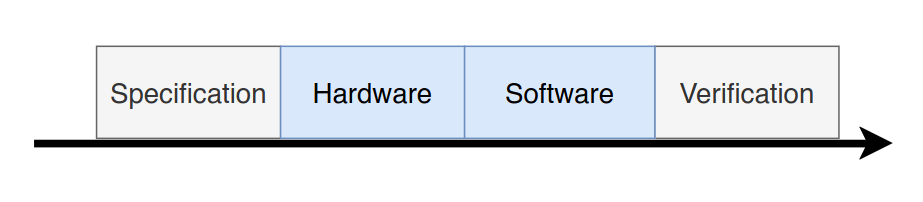
\includegraphics[width=.65\linewidth]{figures/Virtual_platform_without.png}
    \caption{SoC development without virtual platform}
    \label{fig:virtual_platform_without}
\end{figure}

\begin{figure}
    \centering
    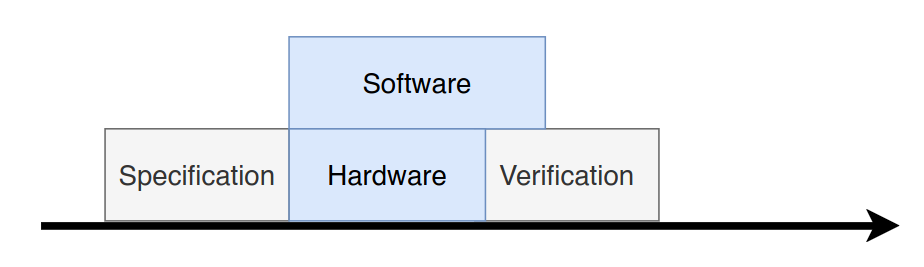
\includegraphics[width=.6\linewidth]{figures/Virtual_platform.png}
    \caption{SoC development with virtual platform}
    \label{fig:virtual_platform}
\end{figure}


\section{Performance Profiling Tools}
Performance profiling plays an important role in software development. In reality, there are always trade-offs between the amount of information available and profiling overhead. Generally speaking, there are two different profiling approaches, namely sampling and instrumentation:

\begin{itemize}
    \item \textbf{Sampling} is the most widely known and the less instrusive approach. Roughly speaking, it collects information about target software application periodically. The most representative sampling-based profiler is linux perf, also known as perf\_event. 
    \item \textbf{Instrumentation} 
\end{itemize}

\chapter{Background}
\section{RISC-V ISA}

RISC-V, which stands for the fifth generation of reduced instruction set computer, was first developed by Krste Asanović in 2010 at UC Berkeley.
Unlike ARM-based microprocessors, RISC-V is an open-source ISA. Hence, it has been considered "the Linux of microprocessors".
As a matter of fact, RISC-V is a lot more than that. The groundbreaking innovation lies in its modular design.

For a long time, incremental ISA, including x86 and ARM, has been the industry convention. In other words, architects keep adding instructions but never removing for the sake of backward compatibility.  
This leads to tremendous complexity in chip design. Besides, hardware costs increase since more silicon areas are required for decode and execution of a wider variety of instructions. And most importantly,
this monolithic design approach introduces less flexibility. There is the analogy - you pay for the whole buffet, but all you want is salad.

\subsection{RV32I Base Integer ISA}
RV32I is the most basic RISC-V ISA, where \texttt{32} indicates 32 bits wide registers and \texttt{I} stands for integer. There are 32 general purpose registers in RV32I, as shown in the upper part of table~\ref{table:riscv_register_calling_convention}. Among those registers, \texttt{x0} is hard-wired to 0, \texttt{x1} is used for holding return address, and \texttt{x10-x17} are used for function arguments.

As shown in fig~\ref{fig:riscv_base_instruction_format}, there are six types of instruction formats:

\begin{itemize}
    \item \textit{R-type} defines register-register operations. Its \texttt{opcode} is \texttt{0110011}. Operands are taken from registers \texttt{rs1} and \texttt{rs2} and result is written into register \texttt{rd}. Common R-type instructions are \texttt{add}, \texttt{sub}, \texttt{sll}, \texttt{slt}, \texttt{sltu}, \texttt{xor}, \texttt{srl}, \texttt{sra}, \texttt{or}, and \texttt{and}.
    
    \item \textit{I-type} defines register-immediate operations. Its \texttt{opcode} is \texttt{0010011}. The 12-bit immediate is sign extended to \texttt{word} and added with register \texttt{rs1}.
    Common I-type instructions are \texttt{addi}, \texttt{slti}, \texttt{sltiu}, \texttt{andi}, \texttt{ori}, and \texttt{xori}. In addition, load instructions, including \texttt{lw}, \texttt{lh}, \texttt{lhu}, \texttt{lb}, and \texttt{lbu}, are also I-type.
    
    \item \textit{S-type} defines store instructions, including \texttt{sb}, \texttt{sh}, and \texttt{sw}. Its \texttt{opcode} is \texttt{0100011}. Data stored in register \texttt{rs2} is stored into target memory address, which is calculated by adding base memory address in register \texttt{rs1} and immediate offset. Note that immediate is split into \texttt{imm[11:5]} and \texttt{imm[4:0]} due to design decision of keeping \texttt{rs1} and \texttt{rs2} in the same place as in R-type.
    
    \item \texttt{B-type} refers to branch instructions, including \texttt{beq}, \texttt{bne}, \texttt{blt}, \texttt{bge}, \texttt{bltu}, and \texttt{bgeu}. Its \texttt{opcode} is \texttt{1100011}. Registers \texttt{rs1} and \texttt{rs2} are compared with each other. If the branch is taken, the new \texttt{pc} is specified by the sum of current \texttt{pc} and \texttt{immediate}. Note that \texttt{imm[0]} is neglected since the RISC-V design specifies that branch offset is always multiples of 2 bytes.
    
    \item \texttt{U-type} refers to \texttt{lui} (load upper immediate) and \texttt{auipc} (add upper immediate to pc). \texttt{lui} deals with large immediate, which I-type instructions cannot handle. For example, in order to load \texttt{0x578ab111} into \texttt{x12}, the two steps are \texttt{lui x12, 0x578ab}, which loads \texttt{0x578ab} into the upper 20 bits and clears the lower 12 bits to 0, then \texttt{add x12, x12, 0x111}.
    
    \item \texttt{J-type} refers to unconditional jump instruction \texttt{jal} (jump and link). Target address is from adding immediate and current \texttt{pc}. Furthermore, since immediate is 21 bits, it can jump to any 16-bit aligned address \texttt{$\pm$1 MB} relative to current \texttt{pc}.
\end{itemize}

\begin{table}
    \centering
    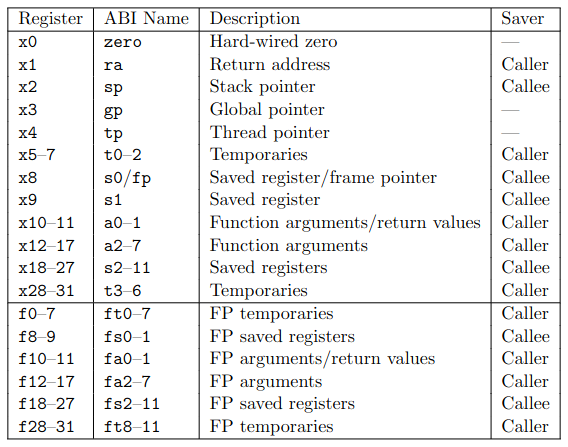
\includegraphics[width=.85\linewidth]{figures/RISCV_register_calling_convention.png}
    \caption{RISC-V register calling convention}
    \label{table:riscv_register_calling_convention}
\end{table}

\begin{figure}
    \centering
    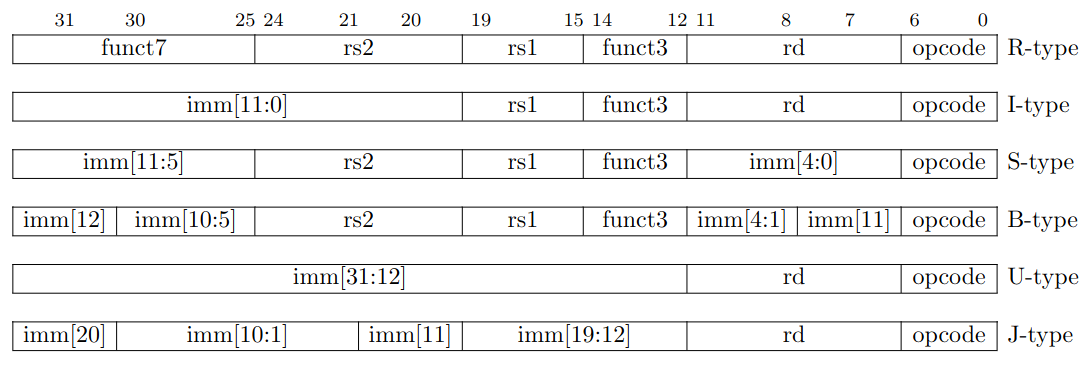
\includegraphics[width=1\linewidth]{figures/RISCV_basic_instruction_format.png}
    \caption{RISC-V instruction format}
    \label{fig:riscv_base_instruction_format}
\end{figure}

\subsection{Standard Extensions}
\begin{itemize}
    \item M refers to integer multiplication and division extension. For multiplication, there are \texttt{mul}, \texttt{mulh}, \texttt{mulhu}, \texttt{mulhsu}, and \texttt{mulw}. For division, there are \texttt{div}, \texttt{divu}, \texttt{divw}, \texttt{divuw}, \texttt{rem}, \texttt{remu}, \texttt{remw}, and \texttt{remuw}.
    
    \item A refers to atomic extension. There are \texttt{lr} (load-reserved), \texttt{sc} (store-conditional), \texttt{amoswap}, \texttt{amoadd}, \texttt{amoand}, \texttt{amoor}, \texttt{amoxor}, \texttt{amomin}, \texttt{amominu}, \texttt{amomax}, and \texttt{amomaxu}.
    
    \item C refers to compressed instructions. Around 50\%-60\% of RISC-V instructions can be compressed. This results in code size reduction of 25\%-30\%.\cite{riscv_manual} 
    
    \item F/D refer to single-precision floating point and double-precision floating point extension respectively.
    
    \item P refers to packed SIMD extension.
    
    \item V refers to vector extension.
\end{itemize}

\section{ETISS}

ETISS, which stands for Extendable Translating Instruction Set Simulator, is developed by TUM EDA chair.
As shown in Figure~\ref{fig:etiss_structure}, it is a C++ instruction set simulator based on dynamic binary translation technique. Furthermore, it features Plugin mechanism for adding new functionalities flexibly.

\begin{figure}[htbp]
    \centering{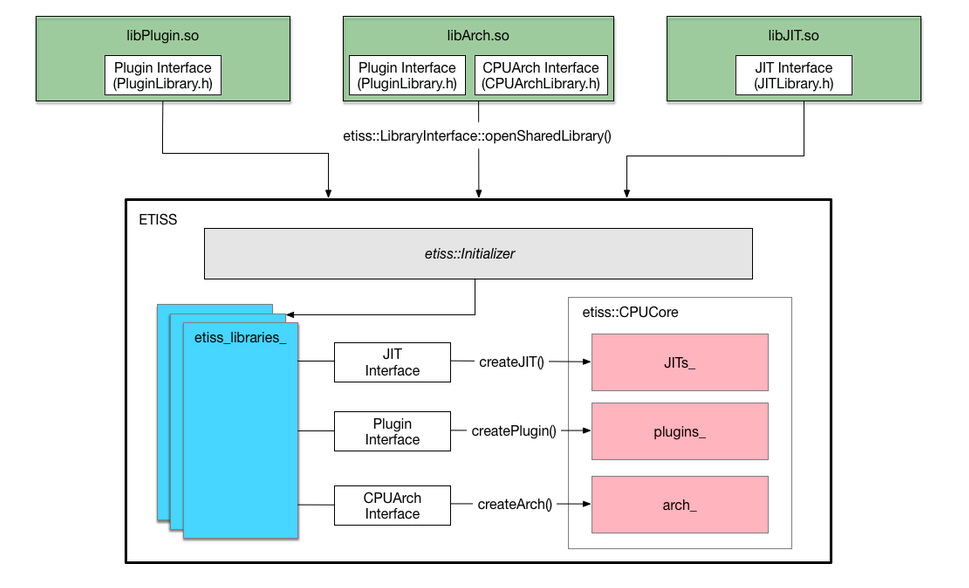
\includegraphics[scale=.4]{figures/ETISS_overview.png}}
    \caption{ETISS structure}
    \label{fig:etiss_structure}
\end{figure}

The following will describe more details on dynamic binary translation and Plugin mechanism respectively.

\subsection{Binary Translation}
Figure~\ref{fig:etiss_binary_translation} illustrates the workflow of dynamic binary translation in ETISS.
First of all, translation block is the atomic unit in binary translator. Program counter is used to check whether the corresponding translation block exists in translation cache.
If not, instructions are fetched starting from current program counter such that a new translation block is loaded. Then, the translation block is translated into C code.
The C code snippet that represents the behaviour of all instructions in a translation block is wrapped as a function in C. The function is compiled into shared library object and cached.
Whenever it is needed, it is loaded into ETISS main loop for execution. 

% Exception handling, interrupts

\begin{figure}[htbp]
    \centering{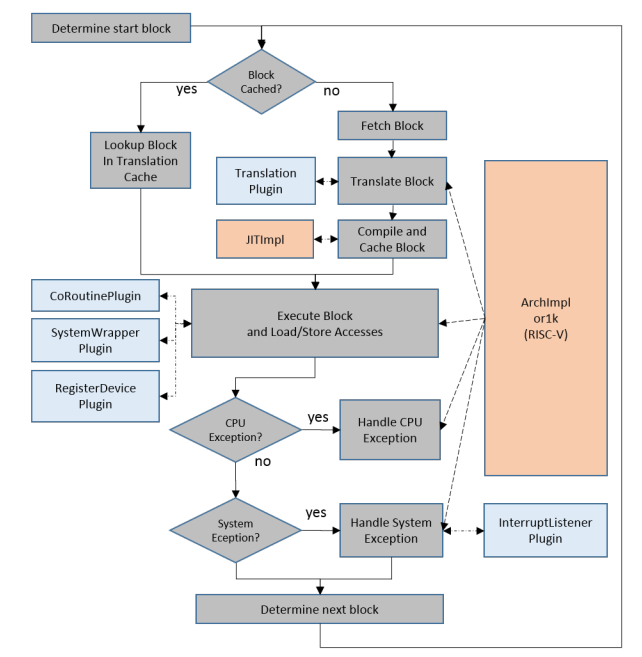
\includegraphics[scale=.45]{figures/ETISS_binary_translation.png}}
    \caption{ETISS Binary Translation}
    \label{fig:etiss_binary_translation}
\end{figure}

\subsection{Plugin Mechanism}
Plugins not only support the core binary translation process but also add functionalities to ETISS based on user's needs without hacking the core ETISS source code.
There are mainly six types of Plugins. For most of the types, an arbitrary number of Plugins can be registered.

\textbf{TranslationPlugin}: TranslationPlugins are executed before translating block. They can be used to add additional C code into translation block and to record the change of state that developers are interested in. Thus, for example, instruction tracing functionality is implemented as TranslationPlugin.

\textbf{CoroutinePlugin}: CoroutinePlugins are executed before the execution of tranlation block. They are mainly used to model closely-coupled peripherals, supporting
interrupt handling and timer functionality.

\textbf{SystemWrapperPlugin}: SystemWrapperPlugins are executed before read/write functions are called. They are mainly used to model load/store behaviours in ETISS framework.

\textbf{RegisterDevicePlugin}: RegisterDevicePlugins serve as the listeners of the architectural registers of interest. As long as register values change, they are notified for further modeling certain parts of closely-coupled peripheral functionalities.

\textbf{ISAPlugin}: One ISAPlugin is registered for each ETISS core. It defines and specifies how instructions are translated and executed in ETISS main loop, including instruction behaviour, instruction binary encoding, and register conventions.

\textbf{JITPlugin}: One JITPlugin is registered for an ETISS instance. It provides the Just-In-Time (JIT) compilation functionality, which compiles C code from translation block into shared libraries.

\section{ELF File}
ELF, which stands for Executable and Linkable Format, is the standard format for executable, relocatable, shared object, and core dump on UNIX-like operating system. The followings are the main components in ELF file.

\subsection{ELF File Header}
\label{subsec:ELF}

ELF file header contains general information of the binary and can be extracted with command line \texttt{\$readelf --header}. An example is shown in fig~\ref{fig:elf_header_example}. It starts with ELF magic number 0x7f and the "ELF" string in ASCII format. And \texttt{Type} can be \texttt{EXEC}, \texttt{REL}, \texttt{DYN}, and \texttt{CORE}. Besides, it indicates pointers to \textit{program headers} and \textit{section headers} and specifies entry point address for executable.

For RISC-V architecture, the \texttt{Flags} field is especially important since it indicates which RISC-V extensions are used and which ABIs should be respected. The layouts are shown in table~\ref{table:elf_header_flags_layout}. 

\begin{table}
    \centering
    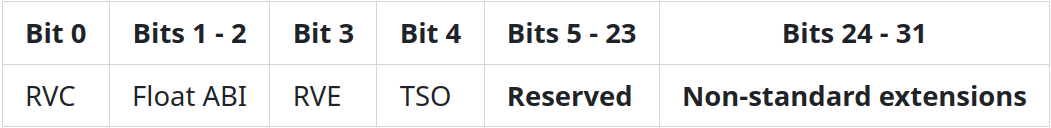
\includegraphics[width=.85\linewidth]{figures/ELF_header_flags_layout.png}
    \caption{Layout of \texttt{Flags} of RISC-V Architecture}
    \label{table:elf_header_flags_layout}
\end{table}

\begin{itemize}
    \item Bit 0 indicates whether C standard extension is used.
    \item Bits 1-2 identify four different floating point ABIs, namely \texttt{SOFT}, \texttt{SINGLE}, \texttt{DOUBLE}, and \texttt{QUAD}.
    \item Bit 3 indicates whether RVE ABI is used.
    \item Bit 4 indicates whether \textit{total store ordering} (TSO) extension is used.
\end{itemize}

\begin{figure}
    \centering
    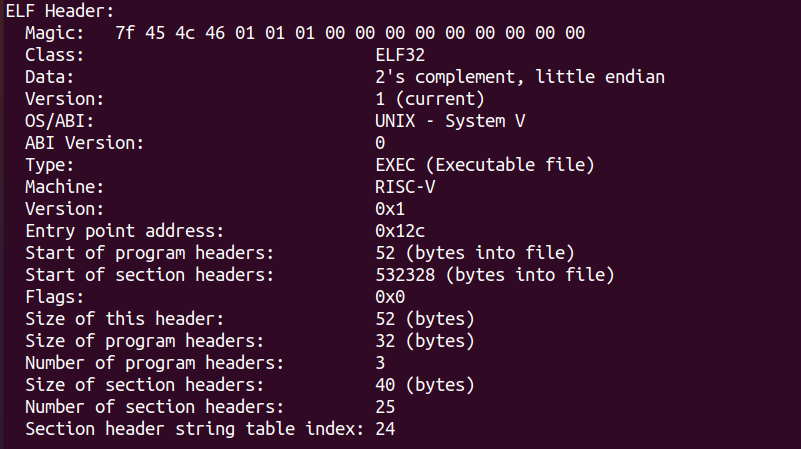
\includegraphics[width=.85\linewidth]{figures/ELF_Header.png}
    \caption{Example of ELF File Header}
    \label{fig:elf_header_example}
\end{figure}

\subsection{Sections and Segments}
ELF is versatile. For linker, sections in ELF are the source of truth. Meanwhile, segments in ELF describe how the binary is processed by loader and kernel. Being said, segments and sections are not orthogonal but interconnected. 

\subsubsection{Segments}
As shown in fig~\ref{fig:elf_program_headers_example}, there are eight fields describing each segment:

\begin{itemize}
    \item \texttt{Type} notifies operating system to load the segment if it is labeled as \texttt{LOAD}. Besides, \texttt{PHDR} means program header and \texttt{INTERP} points out the \textit{dynamic loader} for binary file.
    
    \item \texttt{Offset} refers to byte offset of the segment in ELF file. Linker and loader rely on this information to retrieve correct segment data.
    
    \item \texttt{VirtAddr} and \texttt{PhysAddr} specify where loadable segments should be placed in operating system address space.
    
    \item \texttt{FileSiz} refers to byte size of the segment in ELF.
    
    \item \texttt{MemSiz} refers to byte size of the segment in memory. If \texttt{MemSiz} is greater than \texttt{FileSize}, it means some data is zero-filled and need not be placed in ELF.

    \item \texttt{Flg} specifies permissions. \texttt{R} means readable, \texttt{W} means writable, and \texttt{X} means executable.
    
    \item \texttt{Align} specifies alignment of the segment in memory. Typically, it means the page size of operating system. In the case of fig~\ref{fig:elf_program_headers_example}, it is 4 KB. 
\end{itemize}

\begin{figure}
    \centering
    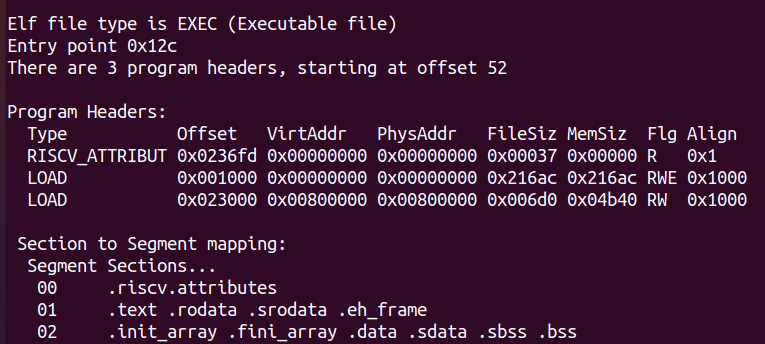
\includegraphics[width=.85\linewidth]{figures/ELF_program_header.png}
    \caption{Example of ELF File Program Header}
    \label{fig:elf_program_headers_example}
\end{figure}

\subsubsection{Sections}

\begin{itemize}
    \item \texttt{.text} is where executable code locates.
    \item \texttt{.rodata} stores read-only data.
    \item \texttt{.data} stores initialized and writable data.
    \item \texttt{.bss} stores zero-initialized and writable data.
    \item \texttt{.symtab} refers to symbol table that stores the mapping between symbols and their locations in ELF, as shown in fig~\ref{fig:elf_symbol_table}. As section~\ref{subsec: elf_info_extraction} will give more details, it is useful for extracting mapping of functions to program counter ranges.
    \item \texttt{.debug\_info} stores main debug information in DWARF format. It appears only when the binary is compiled with \texttt{-g} option.
    \item \texttt{.debug\_line} stores the mapping between program counter and source code line. It also appears only when the binary is compiled with \texttt{-g} option.
\end{itemize}

\subsection{DWARF Format}
DWARF format is the most common debugging format. It is of great importance since GNU debugger (GDB) and LLVM debugger (LLDB) heavily rely on information stored in DWARF-related ELF sections.

DWARF distills information about application program into a tree structure. The tree structure contains multiple \textbf{debugging information entries} (DIEs), which is available by giving the command line \texttt{\$readelf --debug-dump=info <elf file>}. A DIE may have parent DIE, siblings DIEs, or children DIEs. Each DIE contains a \textit{tag} and several \textit{attributes}. \textit{Tag} is the label of a DIE. It can be scope-related, object-related, or type-related. 

\begin{itemize}
    \item Common scope-related \textit{tags}: \textit{compile\_unit}, \textit{namespace}, \textit{subprogram}, \textit{inline\_subroutine},  \textit{label}, \textit{call\_site}, and \textit{lexical\_block} 
    
    \item Common object-related \textit{tags}: \textit{variable} and \textit{formal\_parameter}

    \item Common type-related \textit{tags}: \textit{base\_type}, \textit{typedef}, \textit{array\_type}, \textit{structure\_type}, \textit{union\_type}, \textit{class\_type}, \textit{enumeration\_type}, \textit{subroutine\_type}, \textit{string\_type}, and \textit{subrange\_type}.
\end{itemize}

As for \texttt{attributes}, they may contain constants, variables, or reference to another DIE.~\cite{dwarf}. Several examples are as follows:

\begin{itemize}
    \item \textit{DW\_TAG\_compile\_unit}: As shown in \ref{fig:dwarf_compile_unit}, there are \textit{producer}, \textit{language}, \textit{name}, \textit{comp\_dir}, \textit{low\_pc}, \textit{high\_pc}, \textit{stmt\_list}.
    
    \item \textit{DW\_TAG\_subprogram}: As shown in \ref{fig:dwarf_subprogram}, there are \textit{external}, \textit{name}, \textit{decl\_file}, \textit{decl\_line}, \textit{decl\_column}, \textit{low\_pc}, \textit{high\_pc}, \textit{frame\_base}, \textit{sibling}.

    \item \textit{DW\_TAG\_inlined\_subroutine}: As shown in \ref{fig:dwarf_inlined_subroutine}, there are \textit{abstract\_origin}, \textit{entry\_pc}, \textit{ranges}, \textit{call\_file}, \textit{call\_line}, \textit{call\_column}.

    \item \textit{DW\_TAG\_base\_type}: As shown in \ref{fig:dwarf_base_type}, there are \textit{byte\_size}, \textit{encoding}, and \textit{name}.
\end{itemize}

\begin{figure}
    \centering
    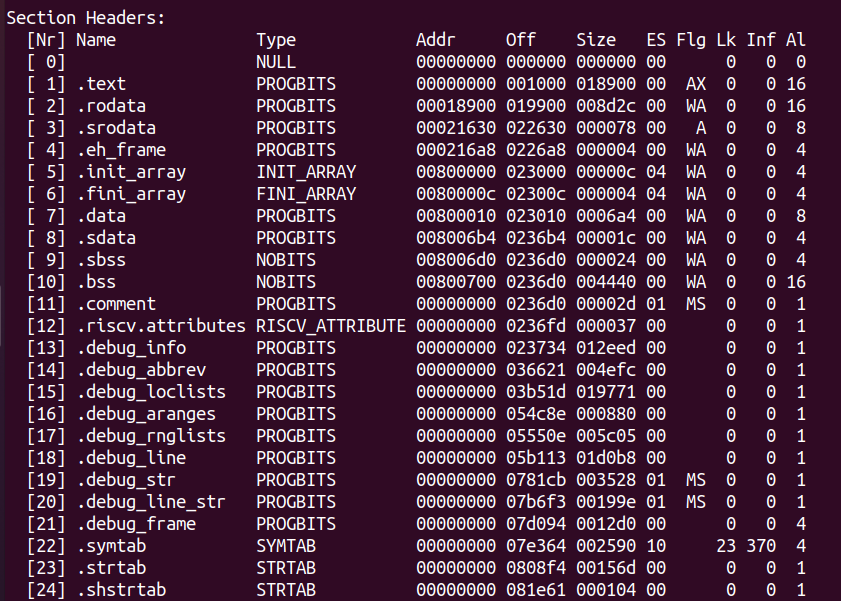
\includegraphics[width=.85\linewidth]{figures/ELF_section_header.png}
    \caption{Example of ELF File Section Header}
    \label{fig:elf_section_headers_example}
\end{figure}

\begin{figure}
    \centering
    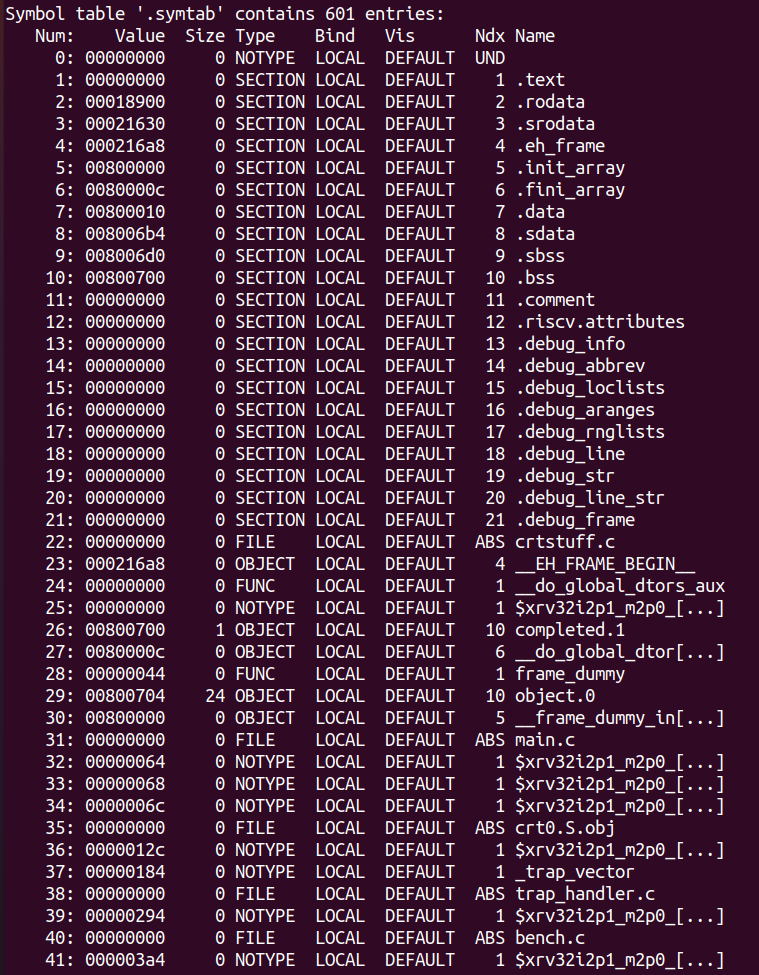
\includegraphics[width=.8\linewidth]{figures/ELF_symtab.png}
    \caption{Example of ELF file symbol table}
    \label{fig:elf_symbol_table}
\end{figure}

\begin{figure}
    \centering
    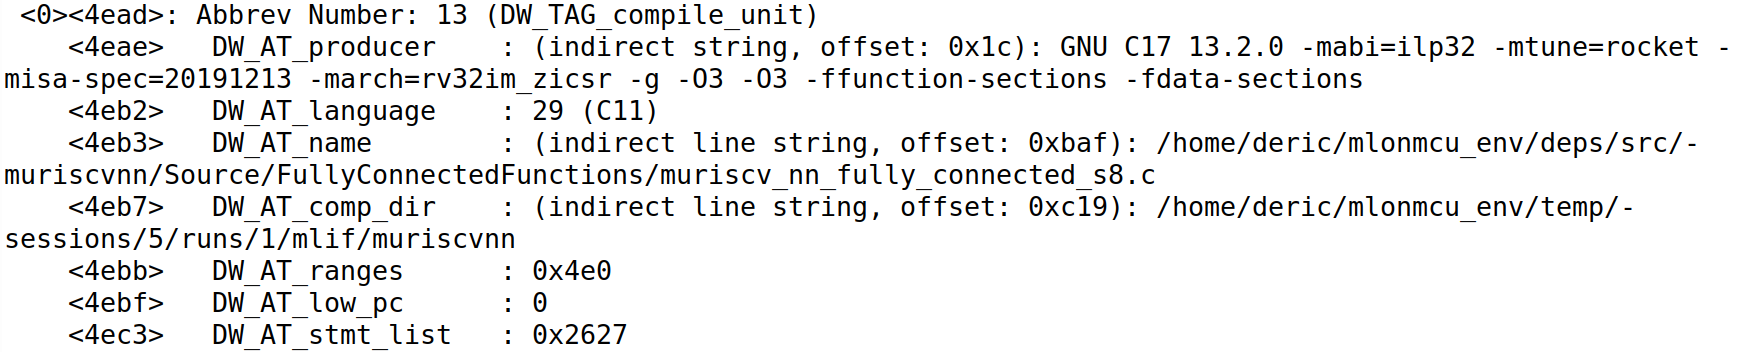
\includegraphics[width=.9\linewidth]{figures/DWARF_compile_unit.png}
    \caption{Example of DWARF compile unit}
    \label{fig:dwarf_compile_unit}
\end{figure}

\begin{figure}
    \centering
    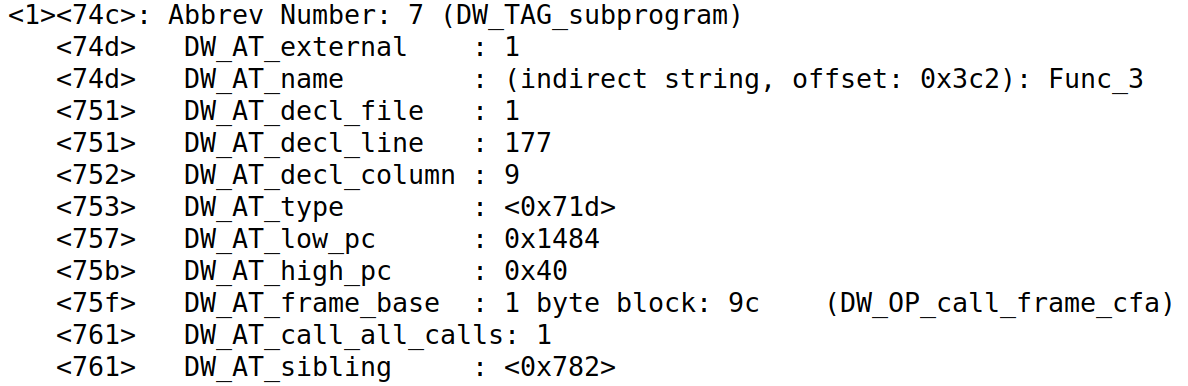
\includegraphics[width=.75\linewidth]{figures/DWARF_subprogram.png}
    \caption{Example of DWARF subprogram}
    \label{fig:dwarf_subprogram}
\end{figure}

\begin{figure}
    \centering
    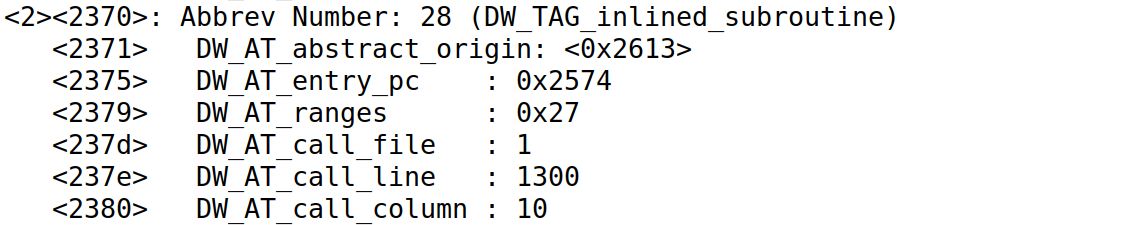
\includegraphics[width=.75\linewidth]{figures/DWARF_inlined_subroutine.png}
    \caption{Example of DWARF inlined subroutine}
    \label{fig:dwarf_inlined_subroutine}
\end{figure}

\begin{figure}
    \centering
    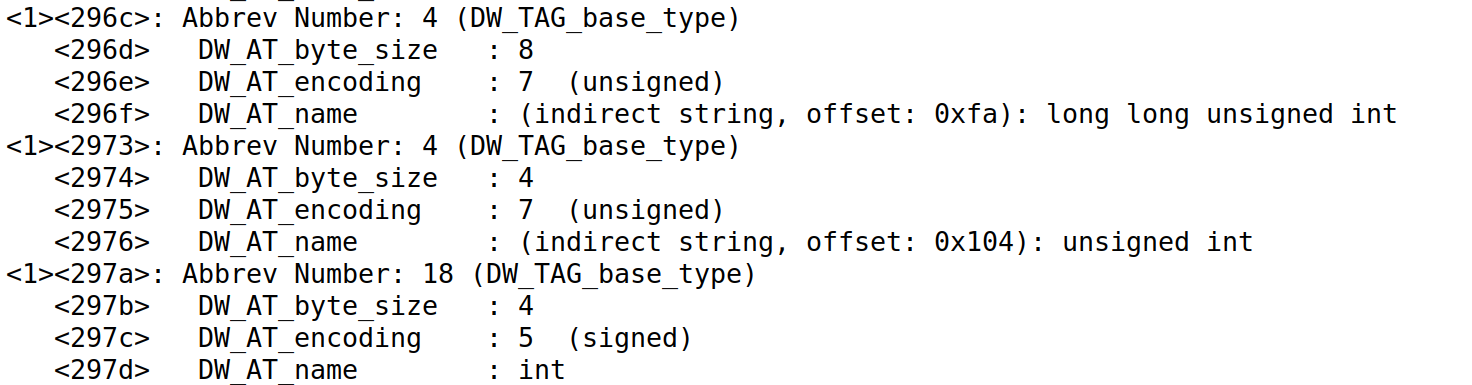
\includegraphics[width=.75\linewidth]{figures/DWARF_base_type.png}
    \caption{Example of DWARF base type}
    \label{fig:dwarf_base_type}
\end{figure}

\subsection{Line Number Table}
\label{subsec:line_table}

Line number table contains the mapping between program counter and corresponding source code. It is stored in ELF \texttt{.debug\_line} section, which is available by giving command line \texttt{\$readelf --debug-dump=line <elf file>}. There are three main components in line number table, namely \textit{directory table}, \textit{file name table}, and \textit{line number statement}.

\begin{itemize}
    \item \textit{Directory table and File name table}: As shown in \ref{fig:dwarf_debug_prologue}, \texttt{File name table} together with \texttt{directory table} clearly show the files and their indices in each directory.
    
    \item \textit{Line number statement}: 
\end{itemize}


\begin{figure}
    \centering
    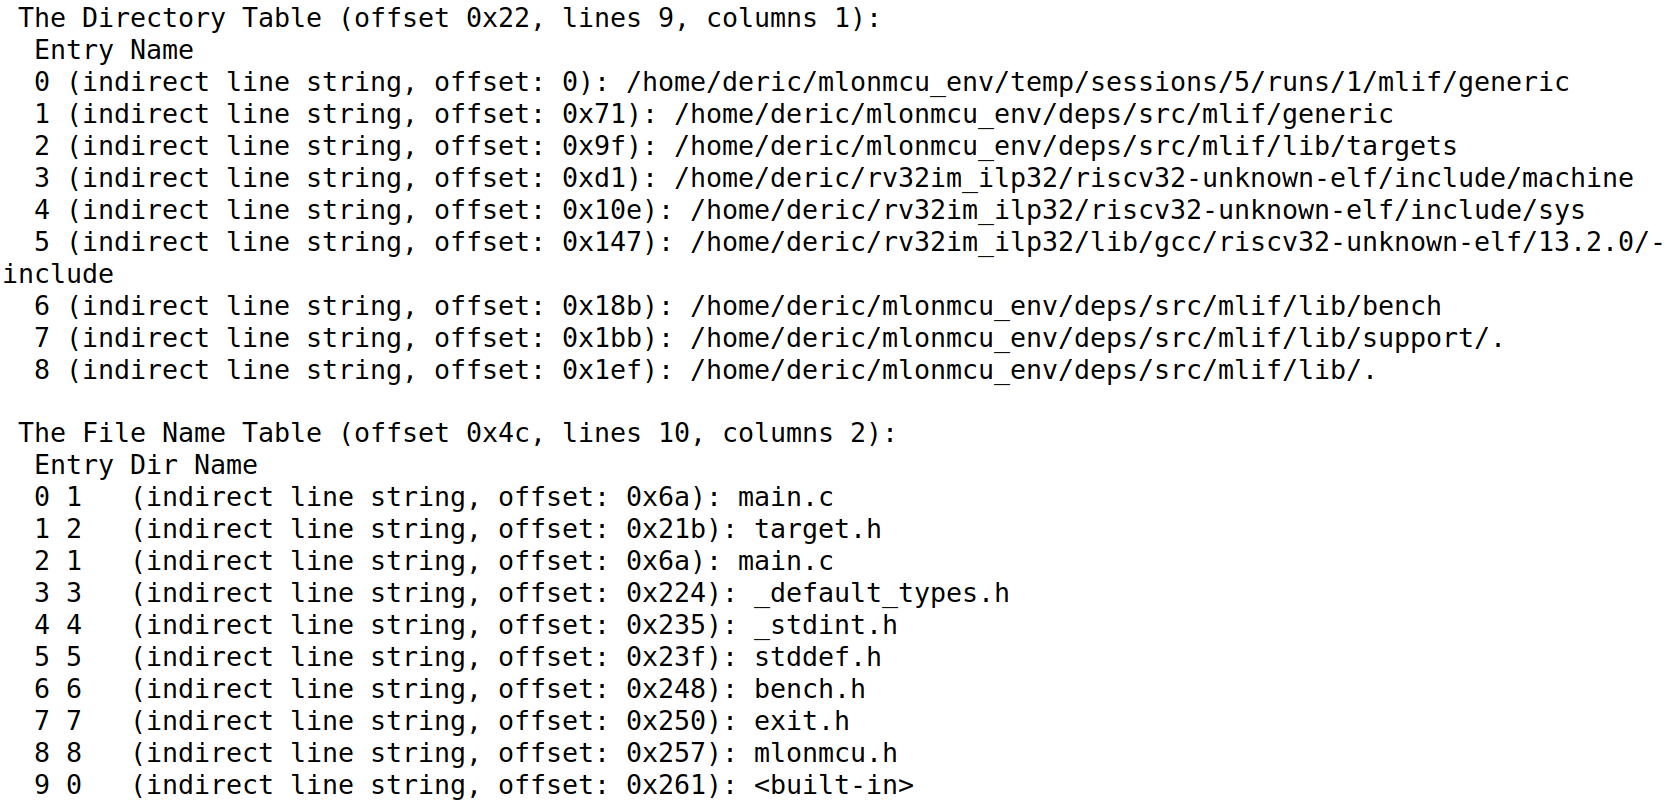
\includegraphics[width=.95\linewidth]{figures/DWARF_debug_prologue.png}
    \caption{Example of DWARF directory table and file name table}
    \label{fig:dwarf_debug_prologue}
\end{figure}

\begin{figure}
    \centering
    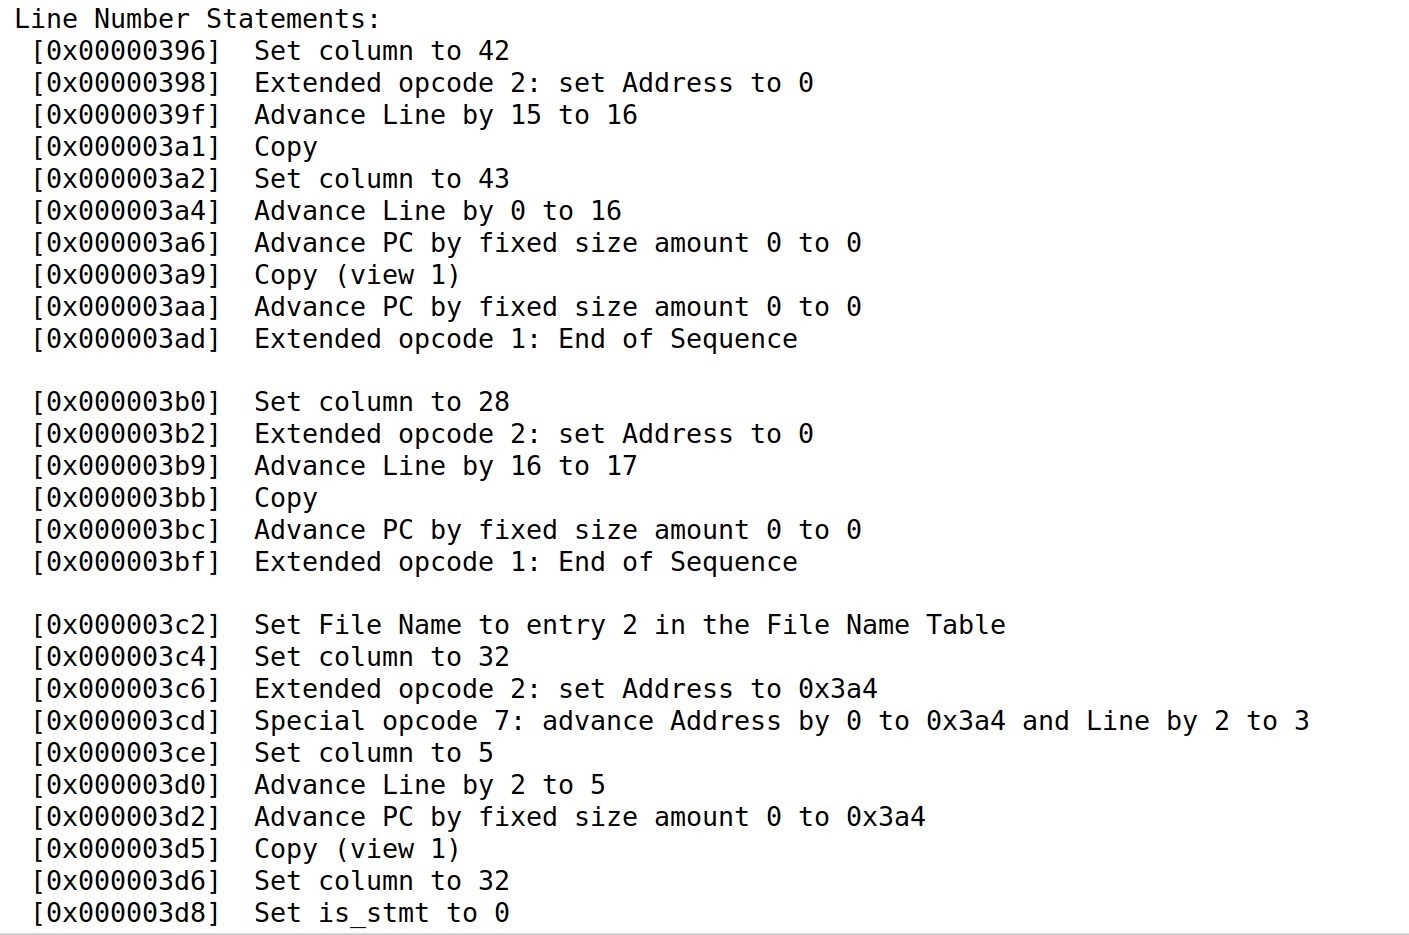
\includegraphics[width=.85\linewidth]{figures/DWARF_debug_main.png}
    \caption{Example of DWARF line number statement}
    \label{fig:dwarf_debug_main}
\end{figure}


\section{Machine Learning Deployment}
Open source deep learning frameworks, such as PyTorch and Tensorflow, are widely known to end users. In contrast, the underlying software stacks that deploy deep learning workloads on diverse hardware backends are less known but extremely crucial. To be more concrete, it is the so-called machine learning compiler that deals with the huge gap between high-level computational graph and binary executable. The following are two widely-used machine learning compiler frameworks.

\begin{figure}
    \centering
    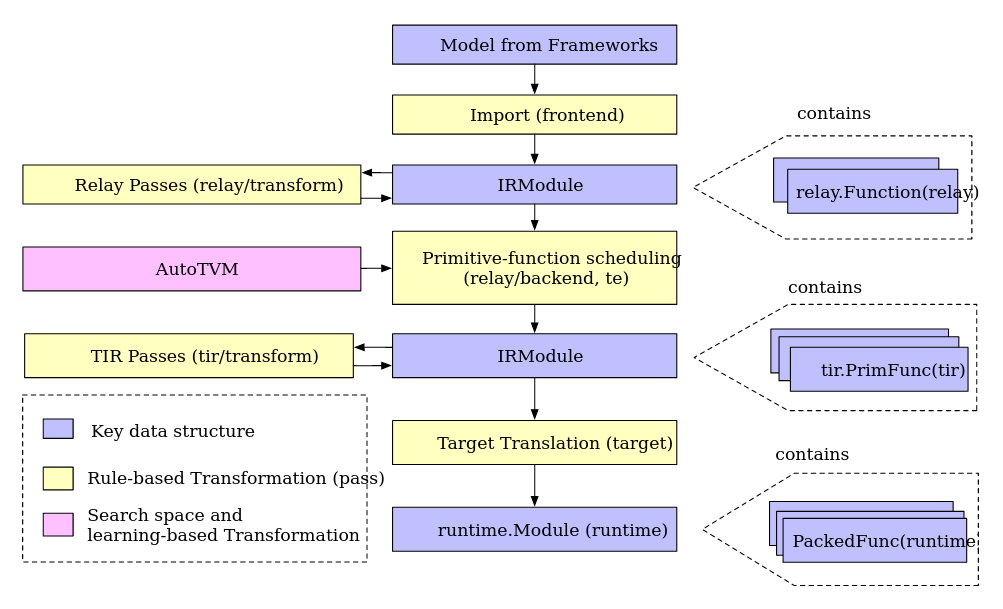
\includegraphics[width=1\linewidth]{figures/TVM_compilation_flow.png}
    \caption{Compilation Flow of TVM}
    \label{fig:tvm_compilation_flow}
\end{figure}

\subsection{TVM}
TVM was developed by a research group at the University of Washington and has evolved into one of the most popular open-source machine learning compiler frameworks. Figure~\ref{fig:tvm_compilation_flow} clearly shows the compilation flow of TVM and its key data structures.

Regarding key data structures, there are two types of intermediate representation (IR), Relay IR and Tensor IR. Relay IR is a high-level functional frontend IR that aims to represent deep learning workloads as computational graphs. On the other hand, Tensor IR is a low-level backend IR for code generation. It represents detailed information about target-specific optimizations on loop structures, memory access patterns, and vector/tensor instructions.

The compilation flow is described in the following.
\begin{enumerate}
    \item It starts with the import of deep learning models of various types and from different frameworks, such as onnx, Tensorflow, PyTorch, and TFLite. The input model is transformed and stored as Relay IRModule.
    \item A collection of Relay passes are responsible for graph-level optimizations. Graph-level optimizations typically include constant-folding, shape inference, canonicalization, dead code elimination, operator fusion and data layout transformation. \textit{Constant-folding} pass identifies graph nodes, of which inputs and outputs are known, precomputes them, then propagates constants through the graph. \textit{Shape inference} pass aims to convert dynamic shapes into static shapes by inferring the inputs and outputs of graph nodes. \textit{Operator fusions} pass aims to fuse multiple operators, minimizing unnecessary data transfer. The predefined seven types of operator, namely elementwise, broadcasting, injective, communicative reduction, complex, tuple, opaque, build the basics of the algorithm.
    \textit{Data layout transformation} pass transforms data layouts into what hardware backend expects or prefers.
    \item AutoTVM is responsible for optimizations that require design-space explorations, such as loop tiling, memory latency hiding, tensorization and many more. In general, the goal is to increase data reuse on the specified hardware backend. However, the fact that there are more and more new machine learning hardware makes the approach of handcrafting each target's characteristics unrealistic. The optimizations in AutoTVM are led by search-based or learning-based algorithms.
    \item 
    
\end{enumerate}

\subsection{MLIR}
MLIR was introduced by Chris Lattner at Google. It is widely used in different domains, including not only machine learning deployment but also quantum computing and query compilation. The main features of MLIR are (1) the flexibility to perform progressive lowering and optimizations at unfixed levels of abstraction, (2) the flexibility to define custom intermediate representation, which is called dialect, and (3) the flexibility to define rewrite patterns in a declarative way.

\subsubsection{IR Design}
An example in figure~\ref{fig:mlir_ir_design} provides an overview of IR design in MLIR. The main components of IR design are dialect, operation, attribute, region, and location information.

\begin{itemize}
    \item \textit{Operation} is the atomic entity in IR. The operation shown in figure~\ref{fig:mlir_ir_design} is \textit{conv2d}. It takes operands \textit{\%input}, \textit{\%filter}, and \textit{\%bias} with types \textit{tensor<1x225x225x3xf32>}, \textit{tensor<32x3x3x3xf32>}, and \textit{tensor<32xf32>} respectively. An operation can have one or more outputs. In this case, it returns \textit{\%0} with type \textit{\%tensor<1x112x112x32xf32>}.
    \item \textit{Attribute} represents compile-time static information of an operation instance. For \textit{conv2d} operation instance in figure~\ref{fig:mlir_ir_design}, attributes are the brace-enclosed key value pairs \textit{\{dilation = [1, 1], pad = [0, 0, 0, 0], stride = [2, 2]\}}. They are kept as a dictionary from string names to underlying values by operation instance. Besides, all attributes are typed.
    \item \textit{Region} enables nested structure inside operation. As illustrated in figure~\ref{fig:mlir_ir_region}, The top-level \textit{for} operation contains a region, where another \textit{for} operation and a terminator \textit{yield} operation exist. Being said, region contains a list of operations, which may also contain regions. This is especially useful for defining structure such as control flow.
    \item \textit{Location information} preserves the source information during the lowering and optimizations process. It is useful for debugging and also for understanding how lowering and optimizations actually work on each operation. 
    \item \textit{Type} is strictly attached to each value in MLIR. There are standard types, including integer, floating point, tensor, vector, memref, tuple and many more. Besides, MLIR type system is extensible to custom dialects and foreign dialects, such as LLVM IR dialect and SPIR-V dialect.
\end{itemize}

Dialect is the container for the above components. It provides granularity for reasoning about the level of abstraction. Common MLIR dialects are shown in figure~\ref{fig:mlir_dialects_overview}. From a high level perspective, MLIR dialects can be categorized through \textit{tensor/buffer} and \textit{payload/structure} axes. \textit{Tensor/buffer} axis indicates whether the dialect of interest mainly deals with \textit{tensor} or \textit{buffer}. The former is typically seen in ML frameworks, whereas the latter is much more relevant to actual memory access. As a result, bufferization is the core of progressive lowering in MLIR, meaning that high-level dialects, such as \textit{onnx-mlir}, \textit{torch-mlir} and \textit{tosa}, are progressively bufferized into lower-level dialects, including \textit{linalg},\textit{memref}, and \textit{arith}. \textit{Payload/structure} axis distinguishes between \textit{what} or \textit{how} computations should be performed. For example, tosa dialect supports common machine learning operators as its operations. However, it doesn't specify how those operators should actually be performed. On the other hand, linalg dialect represents how computations are performed on the structure of interest.

\subsubsection{IR Infrastructure}

IR infrastructure is the core basis that supports IR design. It provides not only great extensiblity to custom dialect design, but also simplifies the usage of MLIR main functionalities from user perspective.

\begin{itemize}
    \item \textit{Operation Descriptions} is supported through TableGen in MLIR. Compared to the usage of C++ template, it is much more intuitive regarding programability, as shown in figure~\ref{fig:mlir_ods}. Moreover, the table-driven manner keeps all the information about the operation of interest in one place such that helper functions generation, verification and analysis for can be done easily.
    
    \item \textit{Rewrite Patterns Declaration} is crucial in MLIR since optimization and lowering rely on this mechanism. The PDL language (PDLL) is a frontend declarative DSL dedicated to pattern matching and rewrite as shown in figure~\ref{fig:mlir_pdll}.
    
    \item \textit{Verifiers} enforce the structure and semantics of IR to be aligned with specification. For example, types should match and terminator operation should exist at the end of each region.
\end{itemize}

\begin{figure}
    \centering
    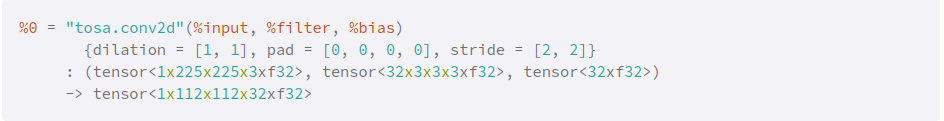
\includegraphics[width=1.\linewidth]{figures/MLIR_IR_design.png}
    \caption{MLIR IR Example}
    \label{fig:mlir_ir_design}
\end{figure}

\begin{figure}
    \centering
    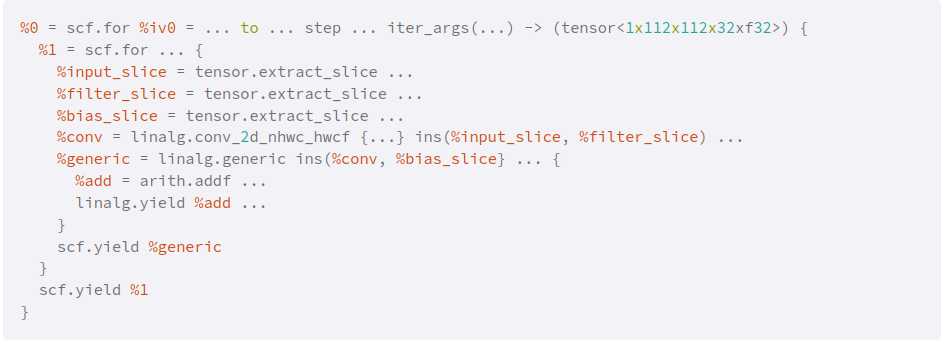
\includegraphics[width=1.\linewidth]{figures/MLIR_IR_region.png}
    \caption{Region in MLIR IR}
    \label{fig:mlir_ir_region}
\end{figure}

\begin{figure}
    \centering
    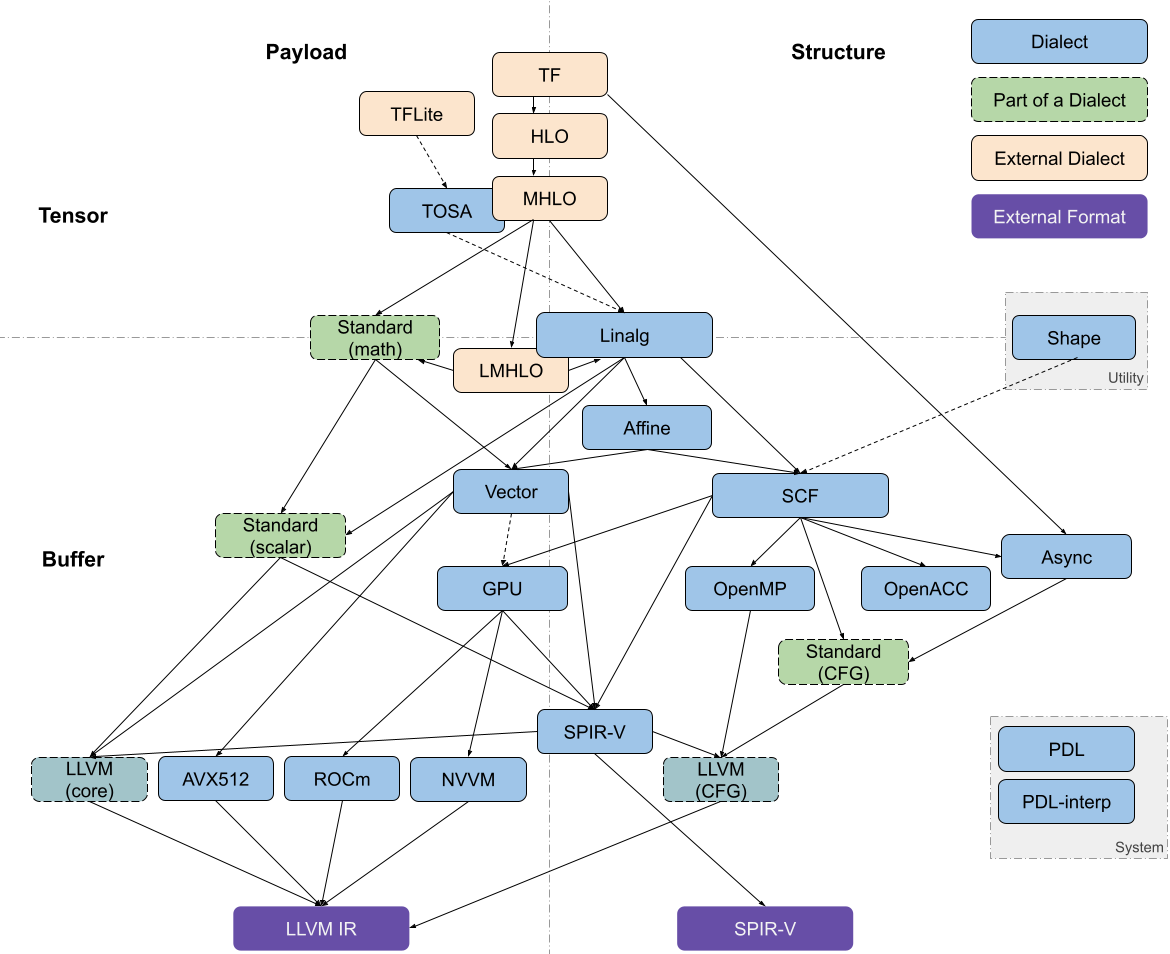
\includegraphics[width=0.8\linewidth]{figures/MLIR_dialect_overview.png}
    \caption{Overview of MLIR Dialects}
    \label{fig:mlir_dialects_overview}
\end{figure}

\begin{figure}
    \centering
    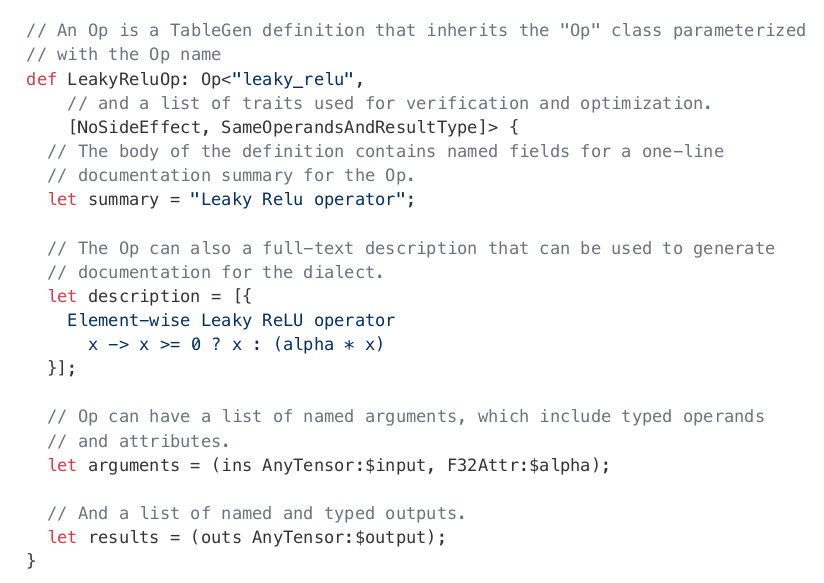
\includegraphics[width=0.8\linewidth]{figures/MLIR_ODS.png}
    \caption{Example of Defining Custom Operation with ODS}
    \label{fig:mlir_ods}
\end{figure}

\begin{figure}
    \centering
    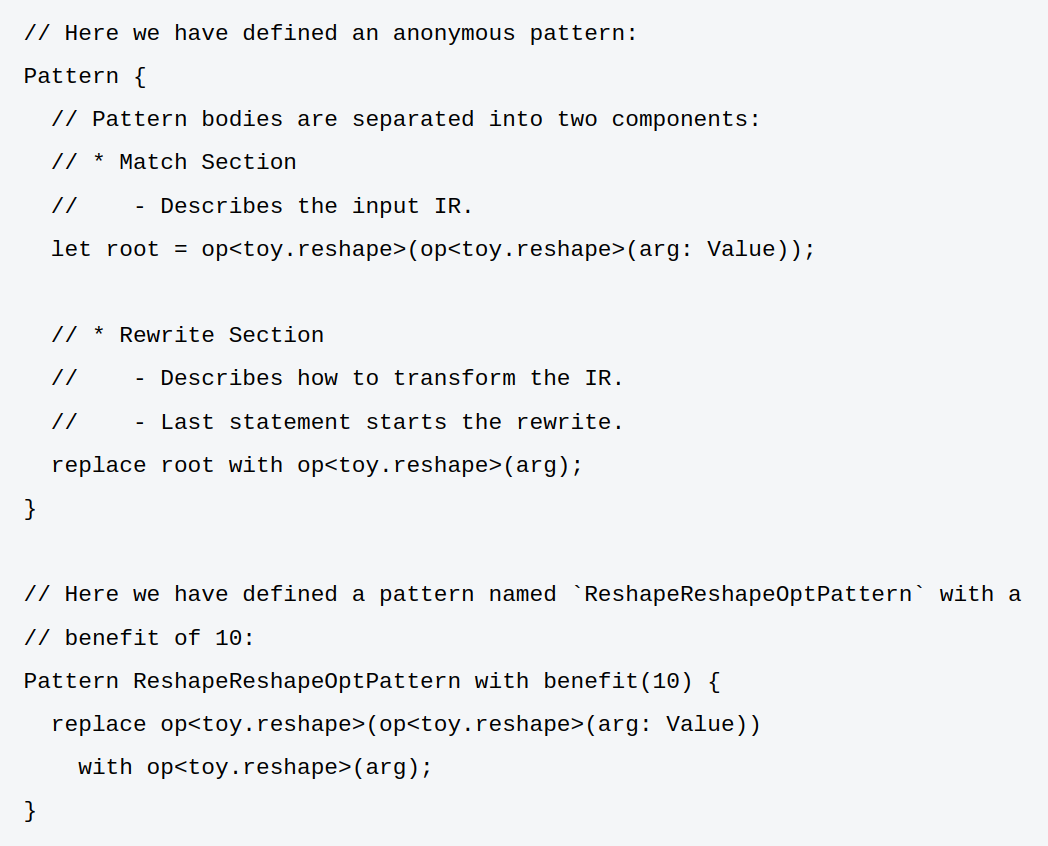
\includegraphics[width=0.6\linewidth]{figures/MLIR_PDLL.png}
    \caption{Example of Declaring Rewrite Patterns with MLIR PDLL}
    \label{fig:mlir_pdll}
\end{figure}

\section{Valgrind}
Valgrind is a widespread software tool for profiling and debugging. To put it in a simple way, it is a virtual machine. The \textit{core} part includes a just-in-time (JIT) compiler and some reimplementations of glibc that deal with signal handling and thread scheduling, whereas the \textit{skin} part is similar to plugin. Custom \textit{skins} can be developed to supervise the aspect of program execution of interest, as long as the \textit{core/skin} interface is respected. Some widely known \textit{skins} are \textit{Memcheck}, \textit{Helgrind}, \textit{ThreadSanitizer}, \textit{Massif}, \textit{Cachegrind}, and \textit{Callgrind}.

\subsection{Core}

\begin{itemize}
    \item JIT compilation: Valgrind internals use \textit{Ucode} as intermediate representation. During binary translation, each basic block is (1) translated to \textit{UCode} format~\ref{fig:valgrind_UCode}, (2) optimized, (3) added with instrumentation, then (3) translated back to x86 instructions~\ref{fig:valgrind_UCode_back}.
    \item Signal Handling: Valgrind intercepts system calls related to signal handling. This way, it can not only fully control application program, but can also mask signals of interest for \textit{skins}.
    \item Thread Scheduling: The \textit{core} has its implementation of pthread functionality. It fully controls thread scheduling, preemption, and synchronization of application program.
\end{itemize}

\begin{figure}
    \centering
    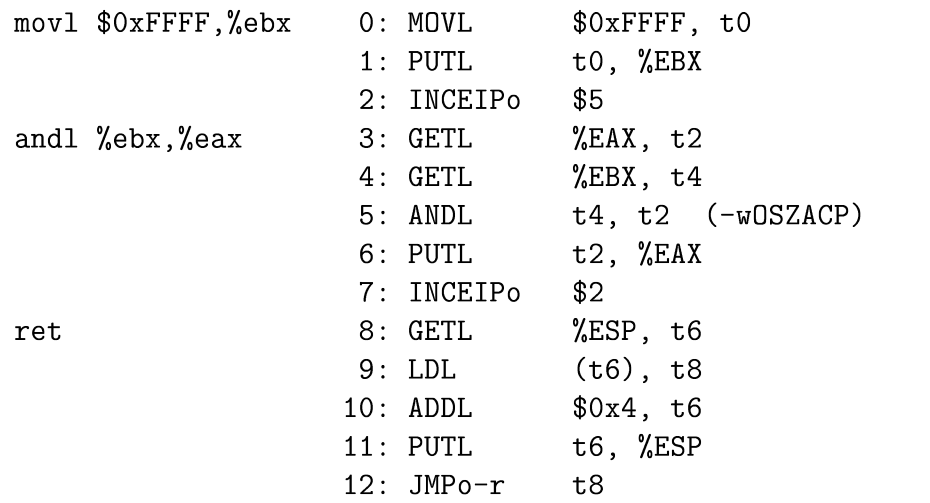
\includegraphics[width=0.55\linewidth]{figures/Valgrind_UCode.png}
    \caption{Instructions are converted to UCode format\cite{valgrind}}
    \label{fig:valgrind_UCode}
\end{figure}

\begin{figure}
    \centering
    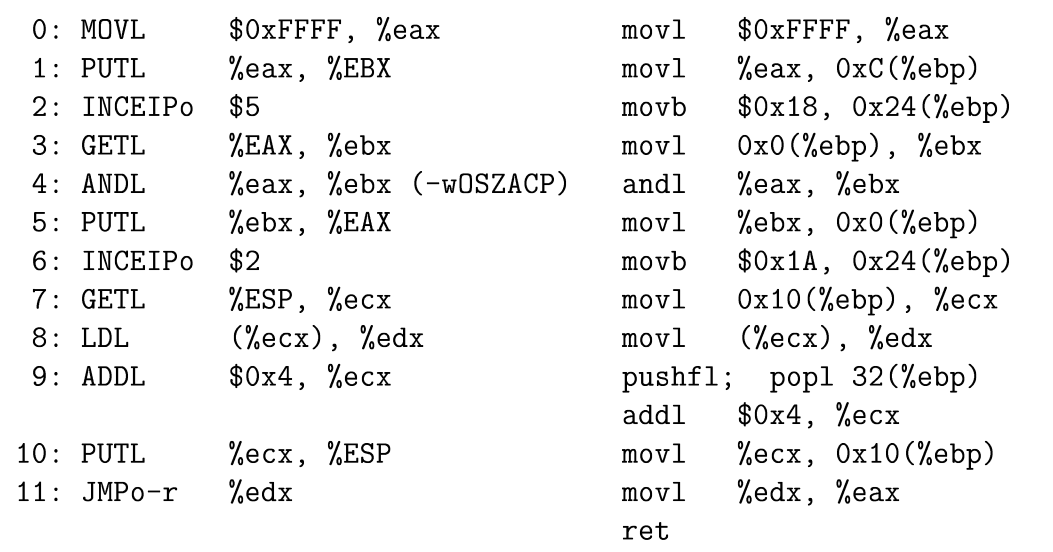
\includegraphics[width=0.55\linewidth]{figures/Valgrind_UCode_2.png}
    \caption{Instructions are converted back to x86 format\cite{valgrind}}
    \label{fig:valgrind_UCode_back}
\end{figure}

\subsection{Core/Skin Interface}
Core/skin interface specifies the APIs for users to develop their own \textit{skins}. Concretely, \textit{vgSkin\_pre\_clo\_init()}, \textit{vgSkin\_post\_clo\_init()}, \textit{vgSkin\_instrument()}, and \textit{vgSkin\_fini()} are the necessary functions of a \textit{skin}. In addition, there are extra structure fields in a \textit{skin} specifying the \textit{core} services, such as error handling, that it wants to subscribe and the events happening in the \textit{core}, such as memory allocation, that it wants to observe. In a nutshell, the design of core/skin interface provides great modularity and extensibility.

\subsection{Common \textit{Skins}}
\label{subsec:callgrind}

\begin{itemize}
    \item \textit{Memcheck} is a memory error detection tool for C/C++ applications, which is capable of reporting memory leaks and illegal memory access in details. This is achieved by maintaining the shadow memory. It represents the real memory with additional \textit{valid-value} and \textit{valid-address} states for each bit. During read/write access or memory allocation, these states are modified accordingly and consulted for errors.
    
    \item \textit{Helgrind} is a thread error detection tool. It is capable of detecting misuses of pthreads API, inconsistent lock orderings, and data races. This is achieved by using happens-before analysis~\cite{happens-before-relation} and lockset algorithm~\cite{lockset-algorithm}. And it turns out that false alarm is part of its nature.
    
    \item \textit{DRD} is also a thread error detection tool. Compared to \textit{Helgrind}, it produces more precise results at the cost of more performance overheads. This is achieved by using vector clocks~\cite{vector-clocks} instead of lockset algorithm.
    
    \item \textit{Massif} is a heap profiler. It is capable of reporting the amount of heap memory used by application program over time. This is achieved by intercepting and tracking \texttt{malloc}, \texttt{free}, \texttt{calloc}, and \texttt{realloc}. In addition, there is a standalone tool Massif-Visualizer for interactive visualization.
    
    \item \textit{Cachegrind} is a memory profiler. It is capable of simulating cache behaviour and branch prediction behaviour and reporting cache utilization, cache hits, and cache misses. This is achieved by maintaining metadata in \textit{global cache state}, \textit{cost center table}, and \textit{instr-info table}~\cite{cachegrind}.
    
    \item \textit{Callgrind} is a performance profiler. It includes all cache simulation features of \textit{cachegrind} and has call graph analysis functionality additionally. Besides, there is a powerful graphical tool \textit{Kcachegrind} for visualizing generated data interactively.
    
\end{itemize}

\subsection{Kcachegrind}
\label{subsec:kcachegrind}

As mentioned in \ref{subsec:callgrind}, \textit{Kcachegrind} is the GUI for callgrind. The main features of \textit{Kcachegrind} are as follow:

\begin{itemize}
    \item \textbf{Multiple Event Types}: \textit{Kcachegrind} visualizes all event types that \textit{callgrind} supports and enables switching between those events at ease. An example is shown in \ref{fig:kcachegrind_caller_callee}.
    
    \item \textbf{Interactive Call Graph}: Call graph is visualized in \textit{Kcachegrind} in an interactive way. Namely, users can not only click on nodes and edges for detailed information, but also use filter to focus on functions of interest. Fig \ref{fig:kcachegrind_treemaps_and_callgraphs} provides an example.
    
    \item \textbf{Source Code/Assembly Annotations}: Metrics of specific event for each line of source code and assembly are annotated right next to each of them. This way, users know, for examples caller-callee relations at the granularity of instruction level or loop structures, without any effort. Fig \ref{fig:kcachegrind_pos_annotations} is an example.
\end{itemize}

\begin{figure}
    \centering
    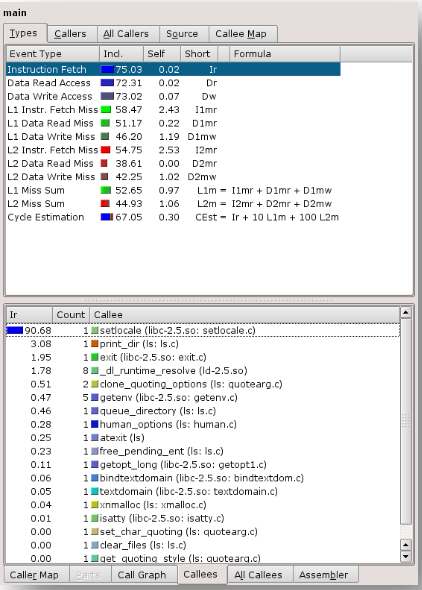
\includegraphics[width=0.65\linewidth]{figures/kcachegrind_caller_callee.png}
    \caption{Lists of event types and callers/callees in Kcachegrind~\cite{kcachegrind}}
    \label{fig:kcachegrind_caller_callee}
\end{figure}

\begin{figure}
    \centering
    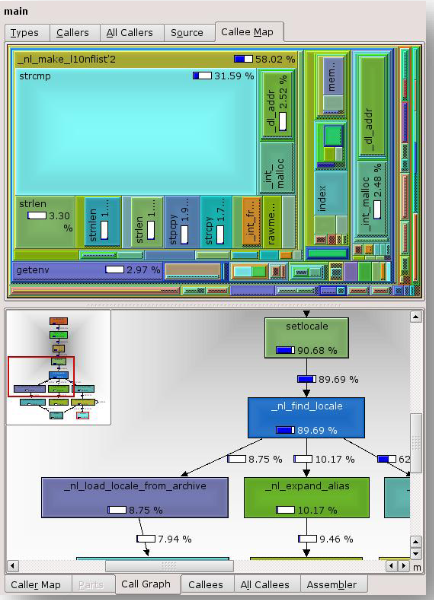
\includegraphics[width=0.65\linewidth]{figures/kcachegrind_callgraph.png}
    \caption{Treemaps and callgraphs in Kcachegrind~\cite{kcachegrind}}
    \label{fig:kcachegrind_treemaps_and_callgraphs}
\end{figure}

\begin{figure}
    \centering
    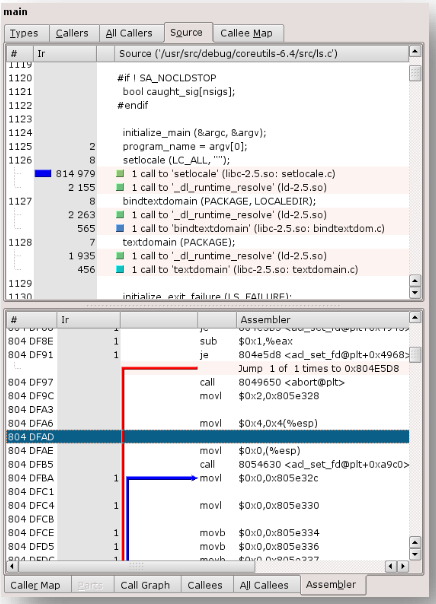
\includegraphics[width=0.65\linewidth]{figures/kcachegrind_pos_annotation.png}
    \caption{Position annotations in Kcachegrind~\cite{kcachegrind}}
    \label{fig:kcachegrind_pos_annotations}
\end{figure}

\chapter{Implementation}
As mentioned in \cref{sec: motivation}, a Python tool has been developed for this work. This chapter highlights its structure and elaborates on the details of its implementation. Besides, several optimization strategies are discussed for improving its performance and memory usage.

\section{Why Python?}

There are mainly two reasons for choosing Python over other compiled languages:

\begin{itemize}
    \item \textbf{Rapid Prototyping}: The fact that Python supports high-level language features makes it simpler to write code and to focus on readability and maintainability. This facilitates rapid prototyping in the scope of this thesis.
    \item \textbf{Rich Libraries Support}: Python has rich libraries support, including file I/O, parsing ELF file, parsing command line options, and matching patterns with regular expressions. As described more in the following sections, all of these libraries are helpful.
\end{itemize}

\section{Workflow}

\begin{figure}[ht]
    \centering
    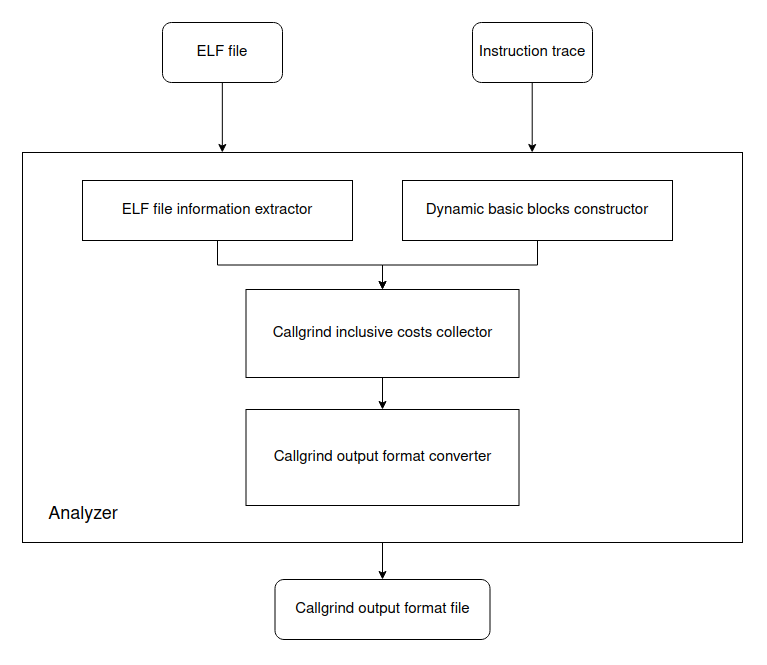
\includegraphics[width=\linewidth]{figures/Analyzer_structure.png}
    \caption{Workflow}
    \label{fig:analyzer_structure}
\end{figure}

\Cref{fig:analyzer_structure} illustrates its structure. An \texttt{Analyzer} object instance takes an ELF file and its ETISS-generated instruction trace as inputs. The \texttt{Analyzer} internals (1) extract information from ELF file, (2) construct dynamic basic blocks, (3) aggregate callgrind inclusive cost, and (4) convert to callgrind output format file. 

\medskip
\dirtree{%
.1 TraceAnalysis/.
.2 main.py.
.2 lib/.
.3 \_\_init\_\_.py.
.3 analyzer.py.
.3 basicBlock.py.
}
\medskip

\subsection{Key Python Objects}

\lstset{
  language=Python,
  basicstyle=\footnotesize\ttfamily,
  breaklines=true,
  frame=single,
  keywordstyle=\color{blue},
  stringstyle=\color{red},
  commentstyle=\color{blue},
  showstringspaces=false,
  captionpos=b
}

\begin{itemize}
    \item \texttt{Analyzer} class is defined in \texttt{lib/analyzer.py}. It is the main class object that takes parameters from command line and performs core functionalities. Four parameters are taken from command line, namely \texttt{elf\_file\_path}, \texttt{trace\_file\_path}, \texttt{dump\_pc}, and \texttt{dump\_pos}. The two latter parameters specify desirable callgrind output format, which will be discussed in  \cref{sec:converter}. Besides, the method \texttt{run} executes internal methods \texttt{\_extract\_ELF\_information}, \texttt{\_build\_basicblocks}, and \texttt{\_callgrind\_output\_format\_converter} consecutively, which will be discussed in the following sections.

    \item \texttt{BasicBlock} class is defined in \texttt{lib/basicBlock.py}. A \texttt{BasicBlock} instance contains variables \texttt{first\_pc}, \texttt{last\_pc}, \texttt{last\_instr}, and \texttt{func}. \Cref{sec:bb_construction} and  \cref{sec:basicblock_optimization} will discussed its usage and possibility for optimization.
\end{itemize}


\medskip
\begin{center}
\begin{minipage}{\textwidth}
\lstset{caption={\texttt{Analyzer} class object}}
\begin{lstlisting}
class Analyzer(object):
    def __init__(self, elf_file_path: str, trace_file_path: str, dump_pc: bool, dump_pos: bool):
    self.elf_file_path = elf_file_path
    self.trace_file_path = trace_file_path
    self.dump_pc = dump_pc
    self.dump_pos = dump_pos

    def run(self, callgrind_output_file_path: str):
        print("=====Extract ELF Information=====")
        self._extract_ELF_information()
        
        print("=====Building Basicblocks=====")
        self._build_basicblocks()

        print("=====Converting To Callgrind Output Format")
        self._callgrind_output_format_converter(callgrind_output_file_path)
        print("=====Conversion Done=====")

    ...
    
\end{lstlisting}
\end{minipage}
\end{center} 

\medskip
\begin{center}
\begin{minipage}{\textwidth}
\lstset{caption={\texttt{BasicBlock} class object}}
\begin{lstlisting}
class BasicBlock(object):
    def __init__(self, first_pc: int, last_pc: int, last_instr: str, func: str):
        self.first_pc = first_pc
        self.last_pc = last_pc
        self.func = func
        self.last_instr = last_instr
    
\end{lstlisting}
\end{minipage}
\end{center}




\subsection{ELF File Information Extraction} 
\label{sec:elf_info_extraction}

The first thing happens inside \texttt{Analyzer} internals is extracting information from ELF files. Specifically, we need to obtain (1) the mapping between static program and dynamic traces, (2) the mapping between source files and functions, and (3) the mapping between program counters and source lines.

\subsubsection{Static Program - Dynamic Traces Mapping}
\label{sec:pc_func_mapping}

Static program and dynamic traces are high-level terms. Concretely, we need the mapping between function and program counter ranges. In Python, there is a well-developed library called \textit{pyelftools}, which is for parsing and analyzing ELF and DWARF debug information.~\cite{pyelftools_manual} The code in \cref{code:func_pc_mapping} uses \textit{pyelftools} to construct this mapping.

With the mapping available, utility function in \cref{alg:query_func_name} queries the function that a program counter of interest belongs to, which is extensively used in \cref{sec:bb_construction} and \cref{sec:converter}.

\medskip
\begin{algorithm}
\caption{Utility function: function name query}
\label{alg:query_func_name}
\begin{algorithmic}
\REQUIRE $pc$, program counter
\REQUIRE $mapping$, mapping between function and program counter range
\FOR{$function$ in $mapping$}
    \IF{$function\_start\_pc \leq pc \leq function\_end\_pc$}
        \RETURN $function\_name$
    \ELSE
        \RETURN $None$
    \ENDIF
\ENDFOR
\end{algorithmic}
\end{algorithm}

\subsubsection{Source Files - Functions Mapping}
Callgrind output format conversion, which will be discussed in section \cref{sec:converter}, requires the mapping between source files and functions. The code in  \cref{code:srcFile_func_mapping} extracts this mapping from DWARF core section using \textit{pyelftools} library. Also, a helper function for retrieving the file name is shown in  \cref{code:helper_function}.

\medskip

\begin{center}
\begin{minipage}[t]{\textwidth}
\lstset{caption={Function that extracts static program - dynamic traces mapping}, label=code:func_pc_mapping}
\begin{lstlisting}[language=Python]
from elftools.elf.elffile import ELFFile

## Assume elf_file_path is given
pc_to_func_mapping = {}

with open(elf_file_path, 'rb') as f:
    elffile = ELFFile(f)

    for section in elffile.iter_sections():
        if section.name == '.symtab':
            symbol_table = section
            break

    for symbol in symbol_table.iter_symbols():
        symbol_type = symbol['st_info']['type']
        if symbol_type = "STT_FUNC":
            start_pc = symbol['st_value']
            end_pc = start_pc + symbol['st_size'] - 1
            pc_to_func_mapping[symbol.name] = (start_pc, end_pc)

\end{lstlisting}
\end{minipage}
\end{center}




\begin{center}
\begin{minipage}{\textwidth}
\lstset{caption={Function that extracts the mapping between source files and functions}, label=code:srcFile_func_mapping}
\begin{lstlisting}[language=Python]
from elftools.elf.elffile import ELFFile
from collections import defaultdict

## Assume elf_file_path is given
srcFiles_to_functions_mapping = defaultdict(list)

with open(elf_file_path, 'rb') as f:
    elffile = ELFFile(f)
    
    dwarfinfo = elffile.get_dwarf_info()
    
    for CU in dwarfinfo.iter_CUs():
        line_program = dwarfinfo.line_program_for_CU(CU)
        if line_program is None:
            continue
    
        for DIE in dwarfinfo.iter_DIEs():
            if DIE.tag == 'DW_TAG_subprogram' \
                and 'DW_AT_decl_file' in DIE.attributes \
                and 'DW_AT_low_pc' in DIE.attributes \
                and 'DW_AT_high_pc' in DIE.attributes:
                func_name = DIE.attributes['DW_AT_name'].value.decode()
                file_idx = DIE.attributes['DW_AT_decl_file'].value
                file_name = lpe_file_name(line_program, file_idx)
                
                if func_name not in self.srcFiles_functions_dict[file_name]:
                    srcFiles_to_functions_mapping[file_name].append(func_name)
\end{lstlisting}
\end{minipage}
\end{center}

\subsubsection{Program Counter - Source Line Mapping}
\label{sec:pc_line_mapping}

As mentioned in \cref{sec:kcachegrind}, kcachegrind supports source code annotations. And this tool is capable of generating \textit{callgrind output format} file ready for this feature. This is achieved by extracting the mapping between program counter and corresponding source code from input ELF file. In section \cref{sec:line_table}, we briefly discuss about the information stored in \texttt{.debug\_line} ELF section, which is all we need. The code in  \cref{code:debug_line_mapping} uses \textit{pyelftools} to extract the mapping for each compilation unit and store all of them in the data structure \texttt{pc\_to\_source\_line\_mapping}. The utility function shown in \cref{alg:query_source_line} relies on the mapping to query source line, which is important in the phase of callgrind output format conversion.

It is worth noting that not every program counter is explicitly recorded in \texttt{.debug\_line} section. For example, the mapping we obtain might look like:

\medskip
\begin{center}
\begin{minipage}{\textwidth}
\lstset{caption={Format of program counter - source line mapping}, label=format:mapping}
\begin{lstlisting}
(0x14, 26)
(0x2b, 27)
(0x30, 28)
...

\end{lstlisting}
\end{minipage}
\end{center}

It means program counters \texttt{(0x14, 0x2b]} are mapped to line 26 and program counters \texttt{(0x2b, 0x30]} are mapped to line 27.

\medskip
\begin{center}
\begin{minipage}{\textwidth}
\lstset{caption={Function that extracts mapping between program counter and source line}, label=code:debug_line_mapping}
\begin{lstlisting}
from elftools.elf.elffile import ELFFile

# Assume elf_file_path is given
pc_to_source_line_mapping = {}

with open(elf_file_path, 'rb') as f:
    elffile = ELFFile(f)

    dwarfinfo = elffile.get_dwarf_info()

    for CU in dwarfinfo.iter_CUs():
        line_program = dwarfinfo.line_program_for_CU(CU)
        if line_program is None:
            continue

        CU_name = CU.get_top_DIE().attributes['DW_AT_name'].value.decode('utf-8')

        for entry in line_program.get_entries():
            if entry.state:
                pc = entry.state.address
                line = entry.state.line
                pc_to_source_line_mapping[CU_name].append((pc, line))
                    

\end{lstlisting}
\end{minipage}
\end{center}

\medskip
\begin{algorithm}
\caption{Utility function: source line query}
\label{alg:query_source_line}
\begin{algorithmic}
\REQUIRE $pc$, program counter
\REQUIRE $source\_file$, source file
\REQUIRE $mapping$, mapping between program counter and source line
\IF{$source\_file$ = None}
    \RETURN None
\ENDIF
\STATE query $mapping$ to get source line
\end{algorithmic}
\end{algorithm}

\subsection{Dynamic Basic Blocks Construction}
\label{sec:bb_construction}

In addition to ELF file, the tool requires user to specify instruction trace file of application program. In particular, the trace generated from ETISS plugin is in the following format:  

\medskip
\begin{lstlisting}
program_counter: instruction_name # binary_encoding_of_instruction operand_field    
\end{lstlisting}

The algorithm is shown in \cref{alg:dynamic_basic_blocks}. First, \texttt{program counter} and \texttt{instruction name} are parsed from the given line in the trace file using Python \texttt{re} library. For an ETISS-generated trace, the usage of \texttt{re} looks like the following:

\medskip
\begin{lstlisting}
pattern = r'(0x[0-9a-fA-F]+):\s*(\w+)\s*#\s*([0-9a-fA-F]+)'
match = re.search(pattern, line) # line in trace file
if match:
    pc = match.group(1)
    instruction = match.group(2)
\end{lstlisting}
\medskip

Afterwards, \texttt{instruction} is checked to see whether it is one of the branch instructions. For the \textit{rv32im\_ilp32} toolchain, these include \texttt{jalr}, \texttt{jal}, \texttt{beq}, \texttt{bne}, \texttt{blt}, \texttt{bge}, \texttt{bltu}, \texttt{bgeu}. If it is true, an instance of the \texttt{BasicBlock} class is constructed. It is worth noting that the design of  \texttt{BasicBlock} object serves the purpose of compressing information from instruction level and providing a larger granularity for the next steps. Moreover, it is not \textbf{static basic block} but more like \textbf{dynamic basic block}. \Cref{fig:basic_block} provides an example. There is a \texttt{BasicBlock} instance with first instruction at \texttt{0x4c08} and last instruction at \texttt{0x4c7c}. At runtime, the branch instruction at \texttt{0x4c7c} sometimes jumps to the middle of that \texttt{BasicBlock} at \texttt{0x4c18}. In this case, a \texttt{BasicBlock} instance with first instruction at \texttt{0x4c18} and last instruction at \texttt{0x4c7c} is also constructed. In other words, a \texttt{BasicBlock} instance can be the superset of any other \texttt{BasicBlock} instance.

One might argue that superset \texttt{BasicBlock} should be split to maintain clear granularity. However, we argue that keeping the superset \texttt{BasicBlock} represents the dynamic trace more explicitly. In addition, this approach simplifies callgrind inclusive cost collection \cref{sec:inclusive_cost} and callgrind output format conversion \cref{sec:converter}. The implementation and optimization details of \texttt{BasicBlock} class will be discussed in \cref{sec:basicblock_optimization}. 

\medskip
\begin{algorithm}
\caption{Dynamic Basic Blocks Construction}
\label{alg:dynamic_basic_blocks}
\begin{algorithmic}
\REQUIRE $dynamic\_basic\_blocks\_list$
\REQUIRE $instruction\_trace$
\FOR{$line$ in $instruction\_trace$}
    \STATE parse $program\_counter$ and $instruction\_name$ from $line$ 
    \IF{$instruction\_name$ is branch instruction name}
        \STATE construct a dynamic basic block instance
        \STATE append the instance into $dynamic\_basic\_blocks\_list$
    \ENDIF
\ENDFOR
\end{algorithmic}
\end{algorithm}
\medskip

\begin{figure}
    \centering
    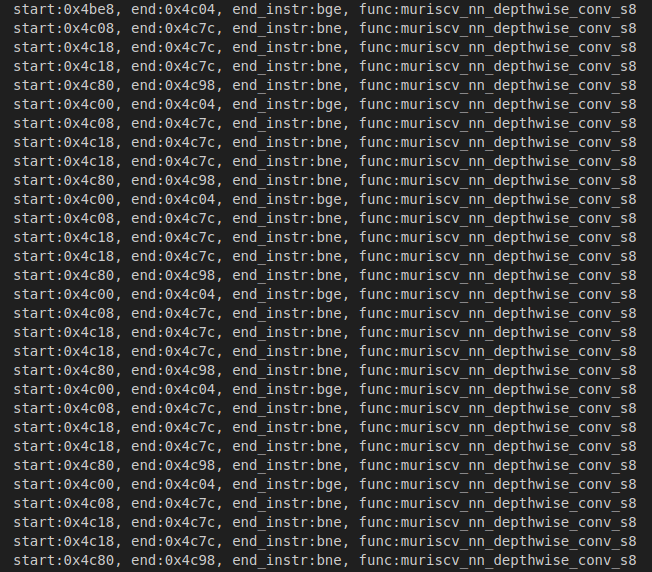
\includegraphics[width=\linewidth]{figures/Basic_Block.png}
    \caption{Example of dynamic basic blocks}
    \label{fig:basic_block}
\end{figure}

\subsection{Callgrind Inclusive Cost Collector}
\label{sec:inclusive_cost}

Inclusive cost includes, taking instruction counts event for example, instructions executed by every child node of the given caller function in the call graph. It is an important source of information for representing caller-callee relationships quantitatively.

\medskip

There are three data structures used for inclusive cost collection:

\begin{itemize}
    \item Call stack: It stores the name of each function in caller-callee relationships.
    \item Basic block stack: It stores \texttt{BasicBlock} instances of each function. In other words, it is a list of lists in Python. 
    \item Inclusive cost dictionary: it stores the mapping between the program counter of branch instruction and the program counter it jumps to together with the corresponding cost. 
\end{itemize}

As shown in \cref{alg:inclusive_cost_collector}, the algorithm iterates over dynamic basic block list mentioned in \cref{sec:bb_construction}. It deals with three cases:

\begin{itemize}
    \item Calling another function: The call stack appends the function name of current basic block, and the basic block stack appends current basic block instance as a Python list.
    \item Jumping inside the same function: The last element in basic block stack appends the current basic block instance.
    \item Returning from a callee: First, the distance between callee and the function it returns to is calculated. Then, the cost is accumulated throughout each caller-callee relationship. Taking the example shown in \cref{fig:analyzer_inclusive_cost}, \texttt{Function B} returns to \texttt{Function A}. Instruction counts for each dynamic basic block in \texttt{Function B} are added up, which are available inside each \texttt{BasicBlock} instance. Besides, the subroutine cost of \texttt{bb3}, which includes all the instruction counts of its subgraph and is annotated in parentheses, is also added up. The accumulation is simply \texttt{56+8+24+16=104} and the resulting number becomes subroutine cost of \texttt{bb1}. At the very end, this iterative procedure yields the inclusive cost dictionary and finally prepare us for generating callgrind output format file. 
\end{itemize}

\medskip
\begin{algorithm}
\caption{Callgrind Inclusive Cost Collector}
\label{alg:inclusive_cost_collector}
\begin{algorithmic}
\REQUIRE $dynamic\_basic\_blocks\_list$
\STATE $call\_stack \gets\ []$
\STATE $bb\_stack \gets\ []$
\STATE $inclusive\_cost\_dictionary \gets\ \{\}$
\STATE $previous\_bb \gets\ None$
\FOR{$current\_bb$ in $dynamic\_basic\_block\_list$}
    \IF{$previous\_bb = None$ or ($previous\_bb.last\_instruction$ is branch instruction and $current\_bb.function \neq prev\_bb.function$)}
        \STATE $call\_stack$.append($current\_bb.function$)
        \STATE $bb\_stack$.append([$current\_bb$])
    \ELSIF{$current\_bb.function = prev\_bb.function$}
        \STATE $bb\_stack$[-1].append($current\_bb$)
    \ELSIF{$previous\_bb.last\_instruction = jalr$}
        \STATE calculate $distance$ between $previous\_bb$ and $current\_bb$
        \FOR{$i$ in range($distance$)}
            \STATE accumulate instruction counts and subroutine cost
        \ENDFOR
    \ENDIF
    \STATE $current\_bb \gets\ previous\_bb$
\ENDFOR
\end{algorithmic}
\end{algorithm}
\medskip

\begin{figure}
    \centering
    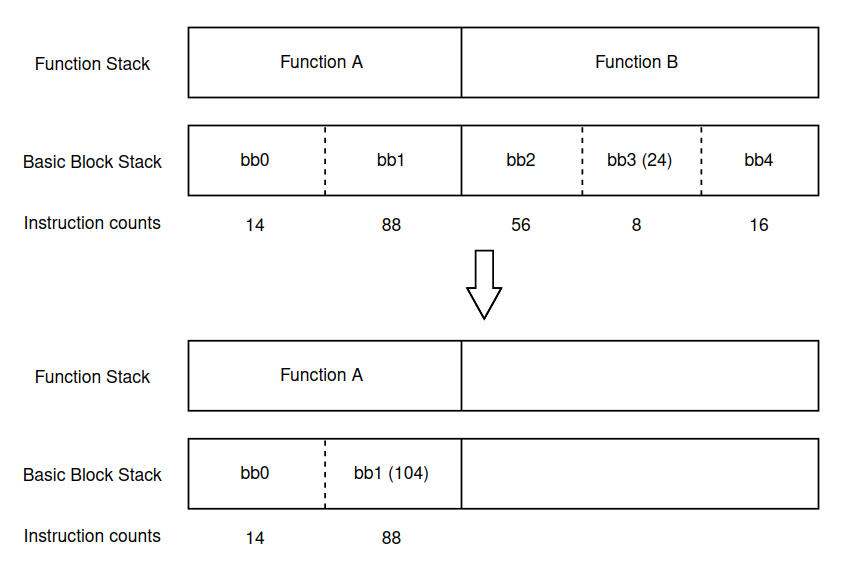
\includegraphics[width=\linewidth]{figures/Analyzer_inclusive_cost.png}
    \caption{Illustration of inclusive cost collection}
    \label{fig:analyzer_inclusive_cost}
\end{figure}
                    
\subsection{Callgrind Output Format Converter}
\label{sec:converter}

Generating callgrind output format file is the last step. The format serves as the common language between callgrind and GUI tool kcachegrind. The full specification won't be discussed here in detail; instead, only the basic structure and the specification for representing caller-callee relationships are important for the scope of this work, which are shown in \cref{code:callgrind_output_format}. First of all, the header should contain magic words \texttt{\# callgrind format}. It should also specify positions and events information. In our case, they are \texttt{positions: instr} and \texttt{events: Instructions}. Regarding general structure, for each function, all of its positions and corresponding cost information are printed in ascending order. As for caller-callee relationships, taking the example in \cref{fig:callgrind_output_format}, the instruction at address \texttt{0x56c} jumps to address \texttt{0x608} for once (\texttt{calls=1}), which belongs to function \texttt{TVMWrap\_GetInputPtr}. And the inclusive cost of \texttt{0x56c} is 6 (\texttt{0x56c 6}).

\lstset{
  basicstyle=\footnotesize\ttfamily,
  breaklines=true,
  frame=single,
  showstringspaces=false,
  captionpos=b
}

\begin{center}
\begin{minipage}{\textwidth}
\lstset{caption={Callgrind output format}, label=code:callgrind_output_format}
\begin{lstlisting}
## header
# callgrind format
version:
creator:
pid:
cmd:

positions: (types of position, e.g. instr and pos)
events: (types of events, e.g. Instructions, Cycles, Flops, and ticks)

## general structure
ob=(ELF file)
fl=(source file)
fn=(function)
(positions) (cost)
...

## example of caller-callee relation
(positions) (cost)
cob=(ELF file of callee)
cfi=(source file of callee)
cfn=(callee function)
calls=(number of calls) (target position)
(positions) (inclusive cost)
\end{lstlisting}
\end{minipage}
\end{center}

\begin{figure}
    \centering
    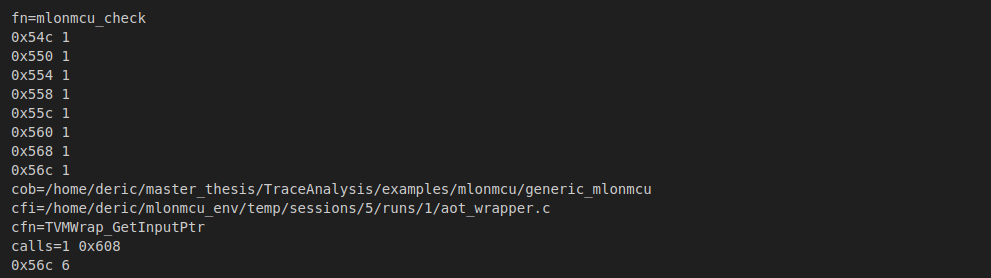
\includegraphics[width=\linewidth]{figures/Output_format_example.png}
    \caption{Example of callgrind output format}
    \label{fig:callgrind_output_format}
\end{figure}

\section{Optimization}
As the workflow and implementation details are shown in previous sections, the question to be asked is - Can we do better? Regarding memory usage of \texttt{BasicBlock} instances and time complexity of the query utility functions, there is indeed room for optimization. 

\subsection{\texttt{BasicBlock} class}
\label{sec:basicblock_optimization}

Recall from \cref{sec:bb_construction} that new \texttt{BasicBlock} instances are constructed over and over again during iterating through instruction trace. However, instances having same values of variables \texttt{start\_pc}, \texttt{last\_pc}, \texttt{last\_instr}, and \texttt{func} should not coexist since they represent same semantics. In fact, for application program that contains many loop structures, especially machine learning applications, original implementation of \texttt{BasicBlock} object wastes too much memory or might even drain RAM space.

Flyweight design pattern comes into play for solving the issue. A common approach is implementing \texttt{BasicBlockFactory} class besides to \texttt{BasicBlock} class. The factory class serves as an interface between client application and original \texttt{BasicBlock} class. It maintains an internal data structure and responds properly to requests. A instance is created only when it doesn't exist in internal data structure.

There is also a more python-oriented approach. In python, \texttt{\_\_new\_\_} and \texttt{\_\_init\_\_} are two important methods for creation and initialization of objects. Static method \texttt{\_\_new\_\_} is called before instance method \texttt{\_\_init\_\_}. As shown in \cref{code:BasicBlock_class}, we can control the process of instance creation in \texttt{\_\_new\_\_}. Namely, an internal data structure \texttt{\_instances} stores the mapping between self-defined key and instance. If the instance exists, \texttt{\_\_new\_\_} directly returns it; otherwise, \texttt{\_\_new\_\_} creates one and returns it.

\Cref{tab:comparison_mem_usage} quantifies the comparison between original implementation and optimization using flyweight design pattern regarding number of \texttt{BasicBlock} instances and their memory usage. Python library \texttt{pymler} is used for inspecting memory usage. It turns that both are reduced by more than 99\% on all four ML models. For smaller models, such as \textit{toycar} and \textit{aww}, this optimization is a nice-to-have. And it becomes a must for larger models such as \texttt{vww} and \texttt{resnet}.

\medskip
\begin{table}[h!]
    \centering
    \resizebox{\textwidth}{!}{
    \begin{tabular}{|c|c|c|c|c|}
    \hline
    \multirow{2}{*}{model}  & \multicolumn{2}{|c|}{original implementation} & \multicolumn{2}{|c|}{with flyweight design pattern} \\
    \cline{2-5}
     & \texttt{BasicBlock} instances & memory usage & \texttt{BasicBlock} instances & memory usage \\
    \hline
     toycar & 99772 & 53.2 MB & 394 & 408 KB \\ 
    \hline
     aww    & 869587 & 564 MB & 669 & 803 KB \\
    \hline
     vww    & 2685142 & 1.4 GB & 765 & 935 KB \\
    \hline
     resnet & 2709481 & 1.41 GB & 617 & 742 KB \\
    \hline
    \end{tabular}
    }
    \caption{Comparison of total memory usage of \texttt{BasicBlock} instances}
    \label{tab:comparison_mem_usage}
\end{table}

\medskip
\begin{center}
\begin{minipage}{\textwidth}
\lstset{caption={BasicBlock class}, label=code:BasicBlock_class}
\begin{lstlisting}
class BasicBlock(object):
    _instances = {}

    def __new__(cls, first_pc: int, last_pc: int, last_instr: str, func: str):
        key = (first_pc, last_pc, last_instr, func)
        instance = cls._instance.get(key)
        if instance is None:
            instance = super().__new__(cls)
            cls._instance[key] = instance
            instance.__initialized = False
            instance._freq = 0
        instance._freq += 1
        return instance

    def __init__(self, first_pc: int, last_pc: int, last_instr: str, func: str):
        if not self.__initialized:
            self.first_pc = first_pc
            self.last_pc = last_pc
            self.func = func
            self.last_instr = last_instr
            self.__initialized = True

\end{lstlisting}
\end{minipage}
\end{center}


\subsection{Query}
Recall from \cref{sec:elf_info_extraction}, there are two utility functions based on program counter to function name mapping and program counter to source line mapping respectively. Given that they are extensively used during dynamic basicblocks construction and callgrind output format conversion, their performance matters. Naively, taking function name query function for example, each key-value pair in \texttt{pc\_to\_func\_mapping} is iterated through in order to find out \texttt{func\_name}, as shown in \cref{code:naive_implementation}. The time complexity turns out to be \( O(n) \). To improve it, binary search comes into play. First of all,\texttt{pc\_to\_func\_mapping} is no longer a python \texttt{dict}; instead, it is a python \texttt{list} that stores \texttt{(start\_pc, end\_pc, func\_name)} as tuple. And it is sorted in ascending order based on \texttt{start\_pc}. Then we use python \texttt{bisect} library to do binary search, as shown in \cref{code:binary_search_func_name}. Similarly, the implementation of source line query function can be optimized by using binary search, as shown in \cref{code:binary_search_source_line}. The resulting time complexity is \( O(\log n) \).



\chapter{Evaluation}
To demonstrate the usefulness of the work, MLonMCU, an automatic end-to-end TinyML benchmarking tool developed by TUM EDA chair, is used. As shown in \cref{fig:evaluation_workflow}, it takes TFLite models from the MLPerf Tiny Benchmark, generates binary executables through TVM compiler with Bring Your Own Codegen (BYOC) framework and RV32IM toolchain, and run binaries on ETISS to generate instruction traces. Then, the implemented tool takes binaries and instruction traces, generating callgrind output format files. Afterwards, profiling results are visualized and evaluated by launching kcachegrind.

It is worth noticing that RISC-V vector extension and packed extension, are not used for evaluation since they are not yet supported by ETISS framework.

\begin{figure}[h]
    \centering
    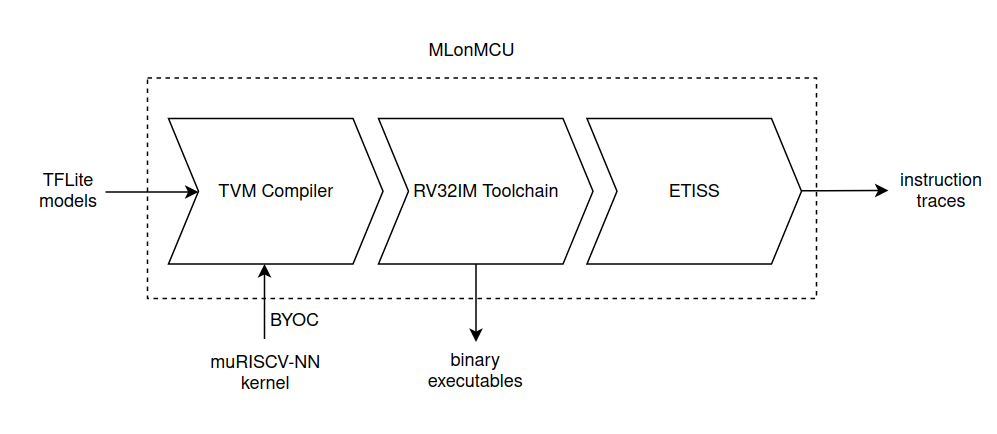
\includegraphics[width=\linewidth]{figures/evaluation_workflow.png}
    \caption{Workflow of using MLonMCU}
    \label{fig:evaluation_workflow}
\end{figure}

\section{Benchmark}
The MLPerf Tiny Benchmark Suite is used for evaluation. As introduced in \cite{banbury2021mlperf}, there are four benchmarks in the benchmark suite:

\begin{itemize}
    \item \textbf{toycar} is related to anomaly detection use case. A FC-AutoEncoder is the model. 
    \item \textbf{aww} is related to keyword spotting use case. A small depthwise-separable DNN is selected as the model.
    \item \textbf{vww} is related to visual wake words use case. MobileNetV1 is selected as the model. 
    \item \textbf{resnet} is related to image classification use case. A customized ResNet-8 is the model.
\end{itemize}

\medskip
\begin{center}
\begin{minipage}{\textwidth}
\lstset{caption={Command lines}, label=code:cmd}
\begin{lstlisting}[language=bash]
# run MLonMCU
$ python3 -m mlonmcu.cli.main flow run <benchmark> --target etiss --backend tvmaotplus
--feature-gen muriscvnnbyoc -c run.export_optional=1 -f log_instrs -c log_instrs.to_file=1 -c riscv_gcc.install_dir=<path to rv32im_ilp32> -c etiss.fpu=none -c etiss.compr
essed=0 -c etiss.atomic=0 -c mlif.debug_symbols=1

# run implemented tool
$ python3 main.py -f <ELF> -t <instruction_trace> --dump-pc=<yes/no> --dump-pos=<yes/no>

# run kcachegrind
$ OBJDUMP=<path of objdump of rv32im_ilp32 toolchain> kcachegrind <output file from implemented tool>
    
\end{lstlisting}
\end{minipage}
\end{center}

\section{Results Analysis}

As described at the beginning of this chapter, command lines for all steps are shown in \cref{code:cmd}. For each benchmark, the muRISCV-NN kernels that are spent most time on during runtime are listed in \cref{tab:benchmark_bottleneck}.

\begin{itemize}
    \item \textbf{toycar} benchmark spends time mostly in \texttt{muriscv\_nn\_vec\_mat\_mult\_t\_s8} kernel. The inner-most loop of the kernel accounts for 94.80\% of kernel instructions.
        
    \item \textbf{aww} benchmark spends time mostly in \texttt{muriscv\_nn\_mat\_mult\_nt\_t\_s8}, \texttt{muriscv \_nn\_depthwise\_conv\_3x3\_s8}, and \texttt{muriscv\_nn\_depthwise\_conv\_s8}. The inner-most loops account for 87\%, 53\% and 72\% instructions of each kernel.
    
    \item \textbf{vww} benchmark spends time mostly in \texttt{muriscv\_nn\_mat\_mult\_nt\_t\_s8}, \texttt{muriscv \_nn\_depthwise\_conv\_s8}. The inner-most loops account for 67\% and 53\% instructions of each kernel.
    
    \item \textbf{resnet} benchmark spends time mostly in \texttt{muriscv\_nn\_mat\_mult\_kernel\_s8\_s16}. The inner-most loop of the kernel accounts for 89.19\% of kernel instructions. 
\end{itemize}

\medskip
\begin{table}[h!]
    \centering
    \resizebox{\textwidth}{!}{
    \begin{tabular}{|c|c|c|c|c|}
    \hline
     benchmark & kernel & relative cost & absolute cost & calls \\
    \hline
    toycar & muriscv\_nn\_vec\_mat\_mult\_t\_s8 & 99.09 & 1,470,894 & 10 \\
    \hline
    \multirow{3}{*}{aww} & muriscv\_nn\_mat\_mult\_nt\_t\_s8 & 61.62 & 9,935,400 & 4 \\ 
    \cline{2-5}
    & muriscv\_nn\_depthwise\_conv\_3x3\_s8 & 23.09 & 3,723,793 & 4 \\
    \cline{2-5}
    & muriscv\_nn\_depthwise\_conv\_s8 & 14.84 & 2,392,755 & 1 \\
    \hline
    \multirow{2}{*}{vww} & muriscv\_nn\_mat\_mult\_nt\_t\_s8 & 68.64 & 31,640,050 & 13 \\ 
    \cline{2-5}
    & muriscv\_nn\_depthwise\_conv\_3x3\_s8 & 23.48 & 10,823,587 & 13 \\
    \hline
    \multirow{2}{*}{resnet} & muriscv\_nn\_mat\_mult\_kernel\_s8\_s16 & 89.19 & 48,640,732 & 2016 \\
    \cline{2-5}
    & muriscv\_nn\_q7\_to\_q15\_with\_offset & 5.43 & 2,959,014 & 31266 \\
    \hline
    \end{tabular}
    }
    \caption{Kernels that account for more than 5\% of total instructions of each benchmark. Cost refers to instruction counts. Relative cost equals absolute cost divided by total number of instructions of specified benchmark.}
    \label{tab:benchmark_bottleneck}
\end{table}

\medskip
\begin{table}[h!]
    \centering
    \resizebox{\textwidth}{!}{
    \begin{tabular}{|c|c|c|c|}
    \hline
    benchmark & kernel & bottleneck(rel) & bottleneck(abs) \\
    \hline
    toycar & muriscv\_nn\_vec\_mat\_mult\_t\_s8 & 94.80\% & 1,394,076 \\
    \hline
    \multirow{3}{*}{aww} & muriscv\_nn\_mat\_mult\_nt\_t\_s8 & 86.98\% & 8,642,304 \\
    \cline{2-4}
    & muriscv\_nn\_depthwise\_conv\_3x3\_s8 & 52.80\% & 1,966,380 \\ 
    \cline{2-4}
    & muriscv\_nn\_depthwise\_conv\_s8 & 78.28\% & 1,872,955 \\
    \hline
    \multirow{2}{*}{vww} & muriscv\_nn\_mat\_mult\_nt\_t\_s8 & 67.50\% & 21,362,944 \\
    \cline{2-4}
    & muriscv\_nn\_depthwise\_conv\_3x3\_s8 & 53.20\% & 5,754,537 \\ 
    \hline
    \multirow{2}{*}{resnet} & muriscv\_nn\_mat\_mult\_kernel\_s8\_s16 & 93.20\% & 45,434,368 \\
    \cline{2-4}
    & muriscv\_nn\_q7\_to\_q15\_with\_offset & 98.91\% & 2,926,848 \\ 
    \hline
    \end{tabular}
    }
    \caption{Bottleneck in kernel. \textbf{bottleneck(abs)} refers to instruction counts of bottleneck part, whereas \textbf{bottleneck(rel)} is \textbf{bottleneck(abs)} divided by total number of instructions of the kernel.}
    \label{tab:muriscv_nn_bottleneck}
\end{table}

\subsection{Possible Optimization Options}
Thanks to kcachegrind, machine code and corresponding source code annotations of bottleneck parts inside critical kernels for each benchmark are available. This enables us to analyze those critical parts directly and to figure out suitable optimization strategies.

It is worth noticing that the quantitative results of instruction counts reduction with each optimization is based on hypothetical estimation. Namely, by looking at machine code and source code annotations side by side in kcachegrind, it is explicit to observe instructions that can be merged or removed and to reason about the numbers.

\subsubsection{Multiply-Accumulate Instruction}
Taking \texttt{muriscv\_nn\_mat\_mult\_nt\_t\_s8} kernel of aww benchmark for example, source line 522, 523, 526, and 527 do multiply-accumulate operations. Multiply-and-accumulate operations in RISC-V P extension are capable of combining \texttt{mul} and \texttt{add} into single instruction. This results in a reduction of 23.5\% of instructions in the critical part (inner-most loop) of the kernel. Results of all kernels concerned are listed in \cref{tab:mac_improvement}.

\begin{figure}[ht]
    \centering
    \begin{minipage}{0.45\textwidth}
        \centering
        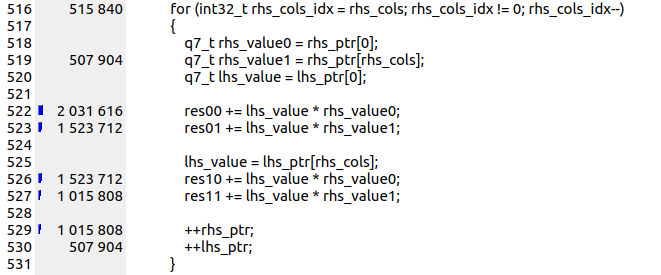
\includegraphics[width=\textwidth]{figures/aww_bottleneck_source_1.png}
    \end{minipage}\hfill
    \begin{minipage}{0.54\textwidth}
        \centering
        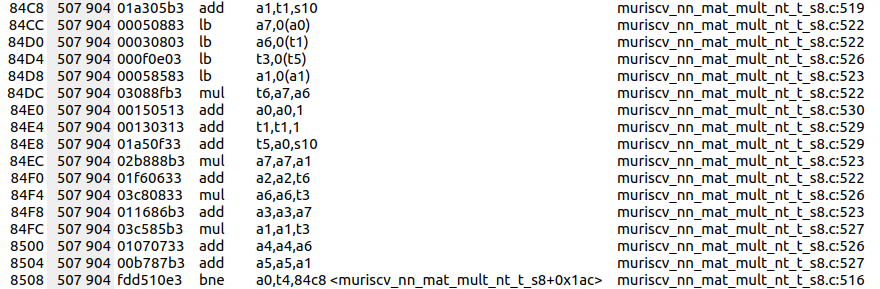
\includegraphics[width=\textwidth]{figures/aww_bottleneck_assembly_1.png}
    \end{minipage}
    \caption{Bottleneck inside \texttt{muriscv\_nn\_mat\_mult\_nt\_t\_s8} kernel for aww benchmark}
    \label{fig:aww_bottleneck}
\end{figure}

\medskip
\begin{table}[h!]
    \centering
    \resizebox{\textwidth}{!}{
    \begin{tabular}{|c|c|c|c|c|}
    \hline
     benchmark & kernel & original & with MAC & reduction \\
    \hline
    toycar & muriscv\_nn\_vec\_mat\_mult\_t\_s8 & 1,394,076 & 1,133,100 & -18.7\% \\
    \hline
    \multirow{3}{*}{aww} & muriscv\_nn\_mat\_mult\_nt\_t\_s8 & 8,642,304 & 6,610,688 & -23.5\% \\ 
    \cline{2-5}
    & muriscv\_nn\_depthwise\_conv\_3x3\_s8 & 1,966,380 & 1,927,980 & -1.95\% \\
    \cline{2-5}
    & muriscv\_nn\_depthwise\_conv\_s8 & 1,872,955 & 1,602,235 & -13.38\% \\
    \hline
    \multirow{2}{*}{vww} & muriscv\_nn\_mat\_mult\_nt\_t\_s8 & 21,362,944 & 15,268,096 & -28.5\% \\ 
    \cline{2-5}
    & muriscv\_nn\_depthwise\_conv\_3x3\_s8 & 5,754,537 & 5,659,305 & -1.65\% \\
    \hline
    \multirow{2}{*}{resnet} & muriscv\_nn\_mat\_mult\_kernel\_s8\_s16 & 45,434,368 & 32,933,376 & -27.51\% \\
    \cline{2-5}
    & muriscv\_nn\_q7\_to\_q15\_with\_offset & 2,926,848 & - & - \\
    \hline
    \end{tabular}
    }
    \caption{Instructions reduction in critical part of each kernel with MAC }
    \label{tab:mac_improvement}
\end{table}


\subsubsection{Post-Incrementing Load/Store}
Post-incrementing load/store instructions perform memory access and increment memory address stored in register by a given offset afterwards. Taking \texttt{muriscv\_nn\_q7\_to \_q15\_with\_offset} kernel in resnet benchmark for example, \texttt{lb a5,0(a0)} and \texttt{add a0,a0,1} can be merged into a single post-incrementing load instruction. Also, \texttt{add a1,a1,2} and \texttt{sh a5,-2(a1)} can be merged into a single post-incrementing store instruction. This results in a reduction of 20.64\% of instructions in the critical part (while-loop) of the kernel. Results of all kernels concerned are listed in \cref{tab:post_increment_improvement}.

\begin{figure}[ht]
    \centering
    \begin{minipage}{0.35\textwidth}
        \centering
        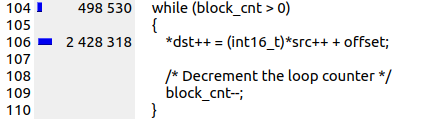
\includegraphics[width=\textwidth]{figures/resnet_bottleneck_source_2.png}
    \end{minipage}\hfill
    \begin{minipage}{0.65\textwidth}
        \centering
        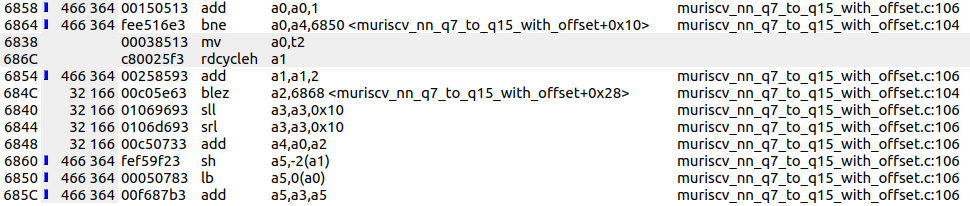
\includegraphics[width=\textwidth]{figures/resnet_bottleneck_assembly_2.png}
    \end{minipage}
    \caption{\texttt{muriscv\_nn\_q7\_to\_q15\_with\_offset} kernel in resnet benchmark}
    \label{fig:resnet_post_increment_example}
\end{figure}

\medskip
\begin{table}[h!]
    \centering
    \resizebox{\textwidth}{!}{
    \begin{tabular}{|c|c|c|c|c|}
    \hline
     benchmark & kernel & original & with post-increment ld/st & reduction \\
    \hline
    toycar & muriscv\_nn\_vec\_mat\_mult\_t\_s8 & 1,394,076 & 1,046,108 & -24.96\% \\
    \hline
    \multirow{3}{*}{aww} & muriscv\_nn\_mat\_mult\_nt\_t\_s8 & 8,642,304 & 7,626,496 & -11.75\% \\ 
    \cline{2-5}
    & muriscv\_nn\_depthwise\_conv\_3x3\_s8 & 1,966,380 & * & * \\
    \cline{2-5}
    & muriscv\_nn\_depthwise\_conv\_s8 & 1,872,955 & * & * \\
    \hline
    \multirow{2}{*}{vww} & muriscv\_nn\_mat\_mult\_nt\_t\_s8 & 21,362,944 & 18,315,520 & -17.27\% \\ 
    \cline{2-5}
    & muriscv\_nn\_depthwise\_conv\_3x3\_s8 & 5,754,537 & * & * \\
    \hline
    \multirow{2}{*}{resnet} & muriscv\_nn\_mat\_mult\_kernel\_s8\_s16 & 45,434,368 & 36,058,624 & -20.64\% \\
    \cline{2-5}
    & muriscv\_nn\_q7\_to\_q15\_with\_offset & 2,926,848 & 1,994,120 & -31.87\% \\
    \hline
    \end{tabular}
    }
    \caption{Instructions reduction in critical part of each kernel with post-incrementing load/store. * means it is difficult to estimate the number hypothetically since for-loop bodies are much more complicated.}
    \label{tab:post_increment_improvement}
\end{table}

\subsubsection{Hardware Loop}
Hardware loop is capable of removing branching and the update of counters and achieves zero-overhead. Taking \texttt{muriscv\_nn\_q7\_to \_q15\_with\_offset} kernel in resnet benchmark for example, \texttt{add a0,a0,1} and \texttt{bne a0,a4,6850} can be replaced with a single hardware loop setup instruction, resulting in a reduction of 31.87\% in the critical part (while-loop) of the kernel. Results of all kernels concerned are listed in \cref{tab:hardware_loop_improvement}.

\medskip
\begin{table}[ht!]
    \centering
    \resizebox{\textwidth}{!}{
    \begin{tabular}{|c|c|c|c|c|}
    \hline
     benchmark & kernel & original & with hardware loop & reduction \\
    \hline
    toycar & muriscv\_nn\_vec\_mat\_mult\_t\_s8 & 1,394,076 & 1,220,092 & -12.48\% \\
    \hline
    \multirow{3}{*}{aww} & muriscv\_nn\_mat\_mult\_nt\_t\_s8 & 8,642,304 & 7,626,497 & -11.75\% \\ 
    \cline{2-5}
    & muriscv\_nn\_depthwise\_conv\_3x3\_s8 & 1,966,380 & * & * \\
    \cline{2-5}
    & muriscv\_nn\_depthwise\_conv\_s8 & 1,872,955 & * & * \\
    \hline
    \multirow{2}{*}{vww} & muriscv\_nn\_mat\_mult\_nt\_t\_s8 & 21,362,944 & 18,315,521 & -17.27\% \\ 
    \cline{2-5}
    & muriscv\_nn\_depthwise\_conv\_3x3\_s8 & 5,754,537 & * & * \\
    \hline
    \multirow{2}{*}{resnet} & muriscv\_nn\_mat\_mult\_kernel\_s8\_s16 & 45,434,368 & 42,309,121 & -6.88\% \\
    \cline{2-5}
    & muriscv\_nn\_q7\_to\_q15\_with\_offset & 2,926,848 & 1,994,121 & -31.87\% \\
    \hline
    \end{tabular}
    }
    \caption{Instructions reduction in critical part of each kernel with hardware loop support. * means it is difficult to estimate the number hypothetically since the for-loop bodies are much more complicated.}
    \label{tab:hardware_loop_improvement}
\end{table}

\subsubsection{Combination of Three Optimizations}
As shown in \cref{tab:total_improvement}, the combination of these three optimizations results in a reduction of instructions around 50\% for matrix-multiply specific kernels. For depthwise specific kernels, it is difficult to provide hypothetical estimations because of the complicated loop structures.

\medskip
\begin{table}[ht!]
    \centering
    \resizebox{\textwidth}{!}{
    \begin{tabular}{|c|c|c|c|c|}
    \hline
     benchmark & kernel & original & all three combined & reduction \\
    \hline
    toycar & muriscv\_nn\_vec\_mat\_mult\_t\_s8 & 1,394,076 & 698,141 & -49.92\% \\
    \hline
    \multirow{3}{*}{aww} & muriscv\_nn\_mat\_mult\_nt\_t\_s8 & 8,642,304 & 5,086,977 & -41.14\% \\ 
    \cline{2-5}
    & muriscv\_nn\_depthwise\_conv\_3x3\_s8 & 1,966,380 & * & * \\
    \cline{2-5}
    & muriscv\_nn\_depthwise\_conv\_s8 & 1,872,955 & * & * \\
    \hline
    \multirow{2}{*}{vww} & muriscv\_nn\_mat\_mult\_nt\_t\_s8 & 21,362,944 & 10,696,961 & -49.93\% \\ 
    \cline{2-5}
    & muriscv\_nn\_depthwise\_conv\_3x3\_s8 & 5,754,537 & * & * \\
    \hline
    \multirow{2}{*}{resnet} & muriscv\_nn\_mat\_mult\_kernel\_s8\_s16 & 45,434,368 & 21,995,009 & -51.59\% \\
    \cline{2-5}
    & muriscv\_nn\_q7\_to\_q15\_with\_offset & 2,926,848 & 1,994,121 & -31.87\% \\
    \hline
    \end{tabular}
    }
    \caption{Instructions reduction in critical part of each kernel with three optimizations combined. * means it is difficult to estimate the number hypothetically since the for-loop bodies are much more complicated.}
    \label{tab:total_improvement}
\end{table}





\chapter{Summary}
This thesis conceptualized and implemented a python tool that enables profiling of tinyML workloads on RISC-V architecture. And by identifying bottlenecks in muRISCV-NN kernels on the MLPerf tiny benchmark suite, the usefulness of this tool is demonstrated regarding three aspects. First of all, the tool is useful since it provides a quick solution to bridge the gap between RISC-V and the existing versatile GUI kcachegrind. Ideally, valgrind that supports RISC-V architecture can provide broader profiling functionalities. However, it is still under active development and there is still a long way to go. In addition, it is useful since it features a clean and simple interface and code hierarchy that is ready to be integrated into ETISS or MLonMCU toolchain. Last but not least, it is useful as we see great potential of extending its functionality to support different aspects of bottleneck identification and performance profiling.

\section{Future Outlook}

There is huge potential to make the implemented profiling tool more versatile and to facilitate development of more RISC-V custom extensions and machine learning kernels. To realize it, several aspects are worth mentioning:

\begin{itemize}
    \item \textbf{Support} RISC-V compressed extension such that the tool could be used in more real scenarios.
    \item \textbf{Support} the collection of cycle counts by leveraging ETISS Performance Estimator.
    \item \textbf{Develop} new functionalities that are capable of collecting information about memory access pattern and even cache utilization of application programs. Being able to provide those information for profiling helps identifying performance bottleneck in a more fine-grained way.
    \item \textbf{Integrate} the work into MLonMCU workflow and bring the benefits of the implemented tool to all the users of MLonMCU. 
    \item \textbf{Open source} the work to RISC-V community since there are only few open-source profiling tools supporting RISC-V architecture, let alone to be simulator-agnostic and with GUI functionality available.  
\end{itemize}

% TODO: add more chapters here

\chapter{Appendix}
\label{chapters:appendix}
\appendix

\section{Appendix A: Examples of DWARF entries}
\begin{figure}[ht]
    \centering
    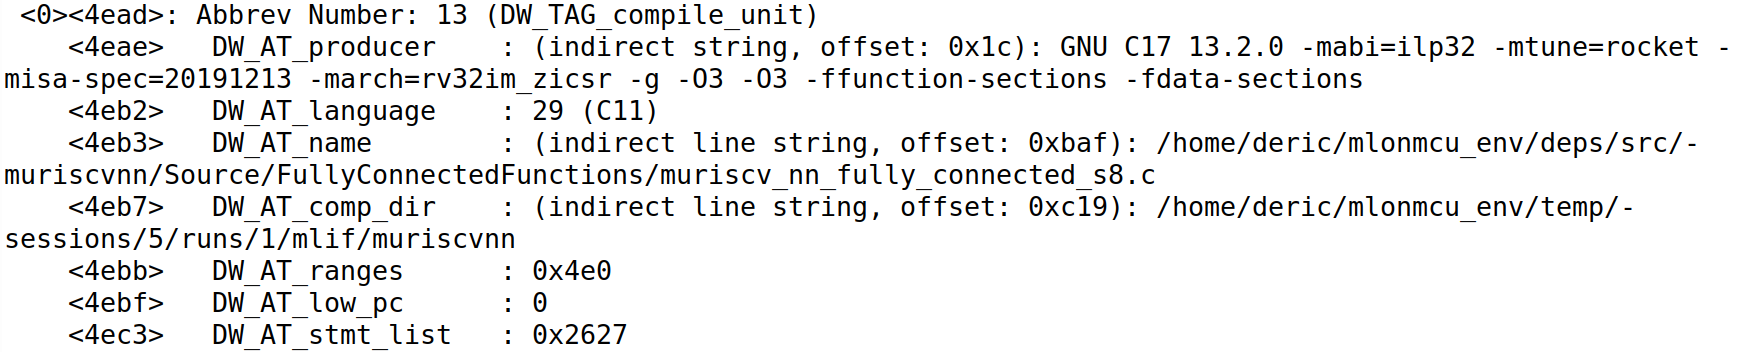
\includegraphics[width=.95\linewidth]{figures/DWARF_compile_unit.png}
    \caption{Example of DWARF compile unit}
    \label{fig:dwarf_compile_unit}
\end{figure}

\begin{figure}[ht]
    \centering
    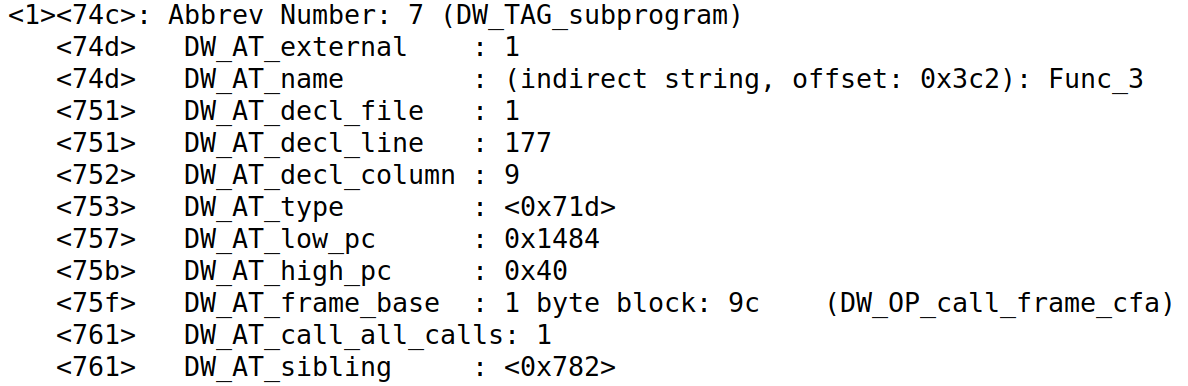
\includegraphics[width=.95\linewidth]{figures/DWARF_subprogram.png}
    \caption{Example of DWARF subprogram}
    \label{fig:dwarf_subprogram}
\end{figure}

\begin{figure}[ht]
    \centering
    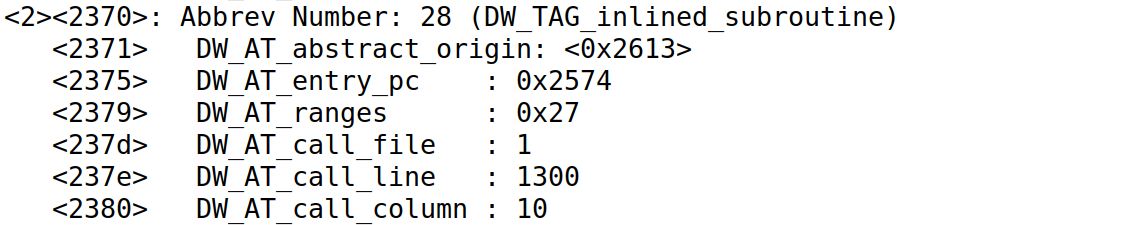
\includegraphics[width=.95\linewidth]{figures/DWARF_inlined_subroutine.png}
    \caption{Example of DWARF inlined subroutine}
    \label{fig:dwarf_inlined_subroutine}
\end{figure}

\begin{figure}[ht]
    \centering
    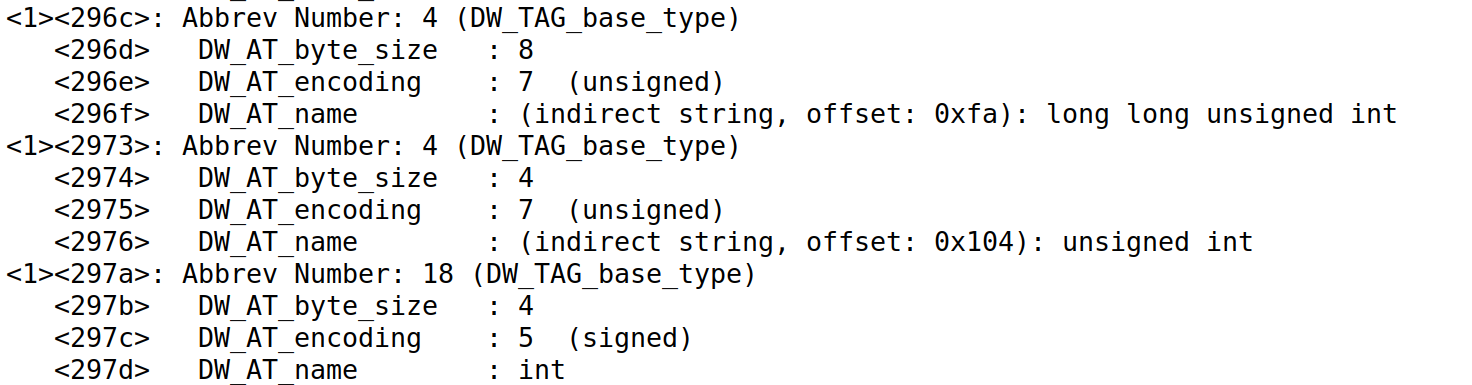
\includegraphics[width=.95\linewidth]{figures/DWARF_base_type.png}
    \caption{Example of DWARF base type}
    \label{fig:dwarf_base_type}
\end{figure}

\begin{figure}[ht]
    \centering
    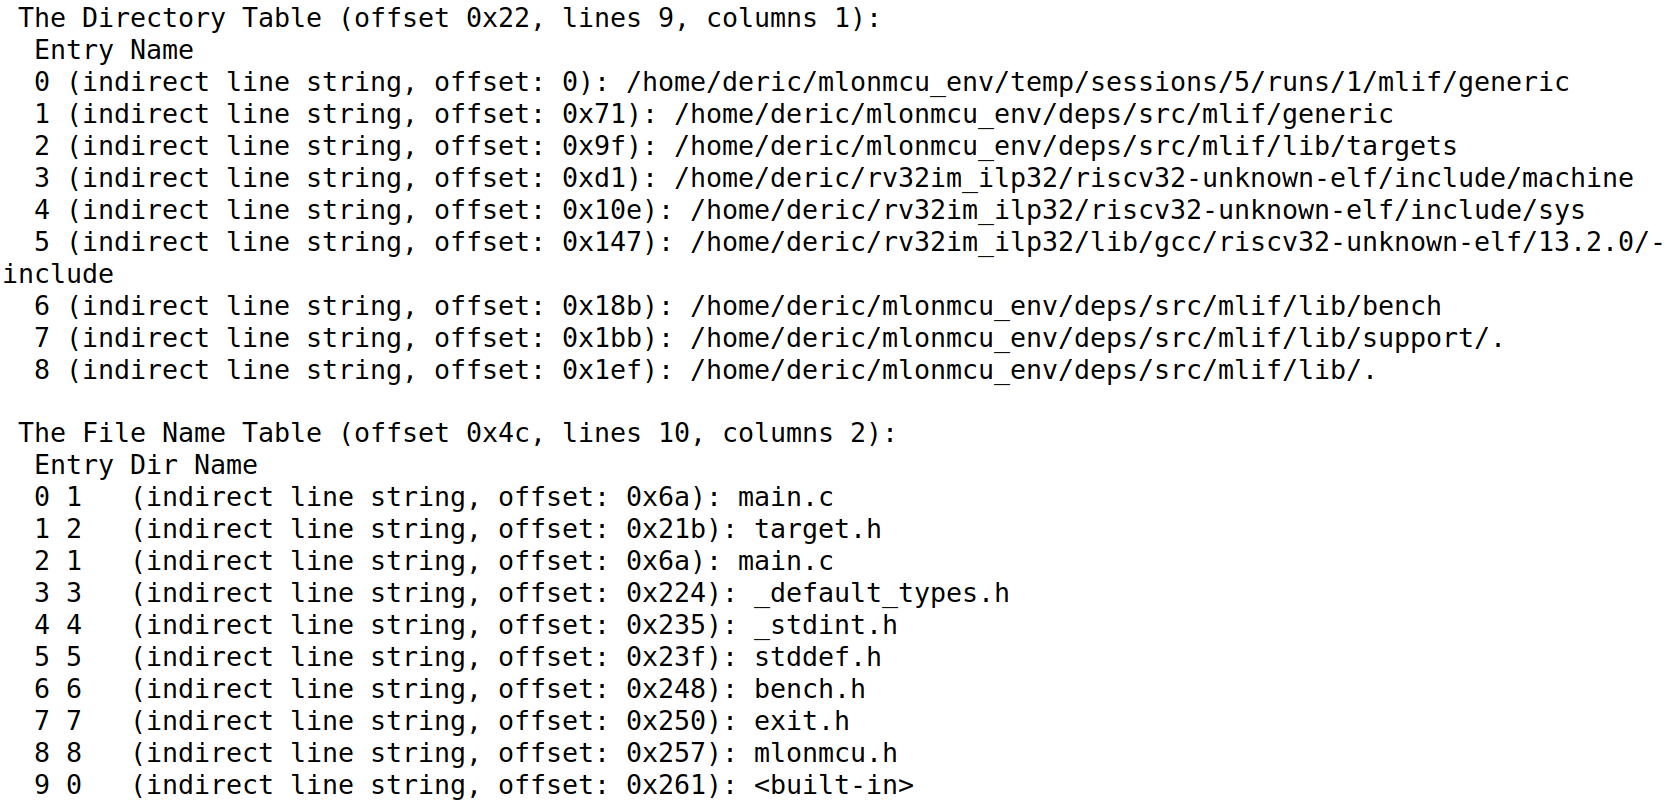
\includegraphics[width=.95\linewidth]{figures/DWARF_debug_prologue.png}
    \caption{Example of DWARF directory table and file name table}
    \label{fig:dwarf_debug_prologue}
\end{figure}

\begin{figure}[ht]
    \centering
    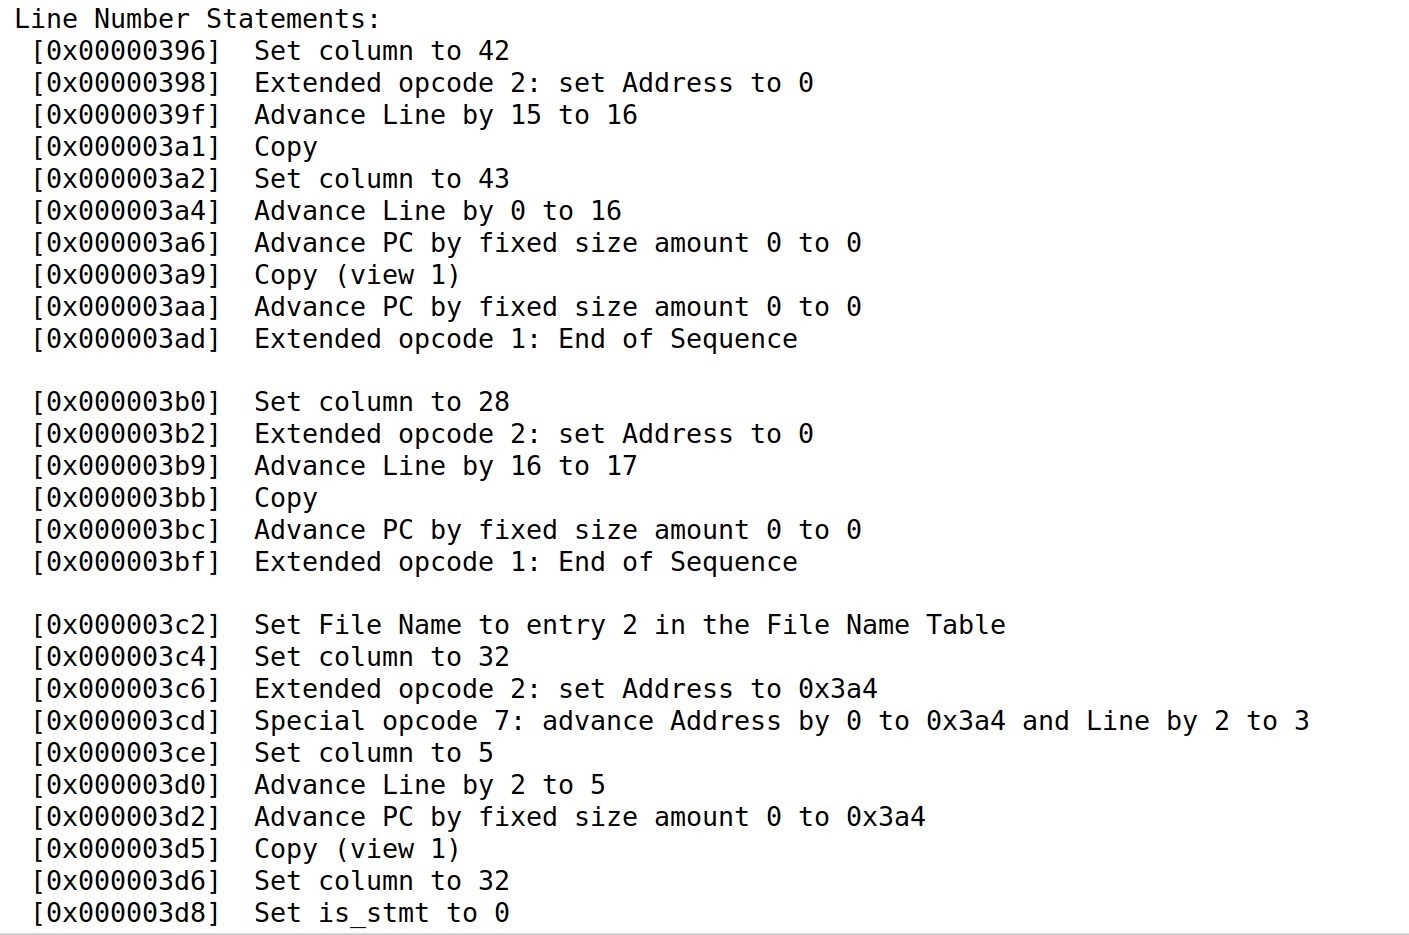
\includegraphics[width=.85\linewidth]{figures/DWARF_debug_main.png}
    \caption{Example of DWARF line number statement}
    \label{fig:dwarf_debug_main}
\end{figure}

\section{Appendix B: Implementation code snippets}
\begin{center}
\begin{minipage}{\textwidth}
\lstset{caption={Helper function for retrieving the file name}, label=code:helper_function}
\begin{lstlisting}
def lpe_filename(line_program, file_idx):
    lp_header = line_program.header
    file_entries = lp_header['file_entry']

    file_entry = file_entries[file_idx] if line_program.header.version >= 5 else \
        file_entries[file_idx-1]
    dir_idx = file_entry['dir_index'] if line_program.header.version >= 5 else \
        file_entry['dir_index'] - 1

    if dir_idx == 0:
        return file_entry.name.decode()

    directory = lp_header['include_directory'][dir_idx]
    return posixpath.join(directory, file_entry.name).decode()
\end{lstlisting}
\end{minipage}
\end{center}


\medskip
\begin{center}
\begin{minipage}{\textwidth}
\lstset{caption={Naive Implementation of \texttt{func\_name} query function}, label=code:naive_implementation}
\begin{lstlisting}
# Assume pc_to_func_mapping is given
# pc_to_func_mapping: {func_name : (start_pc, end_pc)}

def find_func_name(pc: int) -> str:
    for func_name, range in pc_to_func_mapping.items():
        if range[0] <= pc <= range[1]:
            return func_name
    return "???"

\end{lstlisting}
\end{minipage}
\end{center}

\begin{center}
\begin{minipage}{\textwidth}
\lstset{caption={Implementation of \texttt{func\_name} query function by using binary search}, label=code:binary_search_func_name}
\begin{lstlisting}
import bisect

# pc_to_func_mapping is now a list and
# is sorted in ascending order based on start_pc
# pc_to_func_mapping: (start_pc, end_pc, func_name) 
# pc_to_func_mapping.sort(key=lambda x : x[0])

def find_func_name(pc: int) -> str:
    i = bisect.bisect_right(pc_to_func_mapping, pc, key=lambda x : x[0])
    if i > 0:
        start_pc, end_pc, func_name = pc_to_fun_mapping[i-1]
        if start_pc <= pc <= end_pc:
            return func_name
    return "???"
    
\end{lstlisting}
\end{minipage}
\end{center} 

\begin{center}
\begin{minipage}{\textwidth}
\lstset{caption={Implementation of source line query function by using binary search}, label=code:binary_search_source_line}
\begin{lstlisting}
import bisect

# pc_to_source_line_mapping : {source_file : [(pc, source_line), ...]}
# Asssume pc_to_source_line_mapping is given and
# , for each source file, the list is sorted in ascending order
# based on pc

def dump_source_line(pc: int, source_file: str) -> str:
    if source_file == "???":
        return "0"
    mapping = pc_to_source_line_mapping[source_file]
    i = bisect.bisect_right(mapping, pc, key=lambda x : x[0])
    if i > 0:
        start_pc, line = mapping[i-1]
        if pc >= start_pc:
            return f"{line}"
    return "0"

\end{lstlisting}
\end{minipage}
\end{center}

\section{Appendix C: Callgraph of benchmarks}
\begin{figure}[ht]
    \centering
    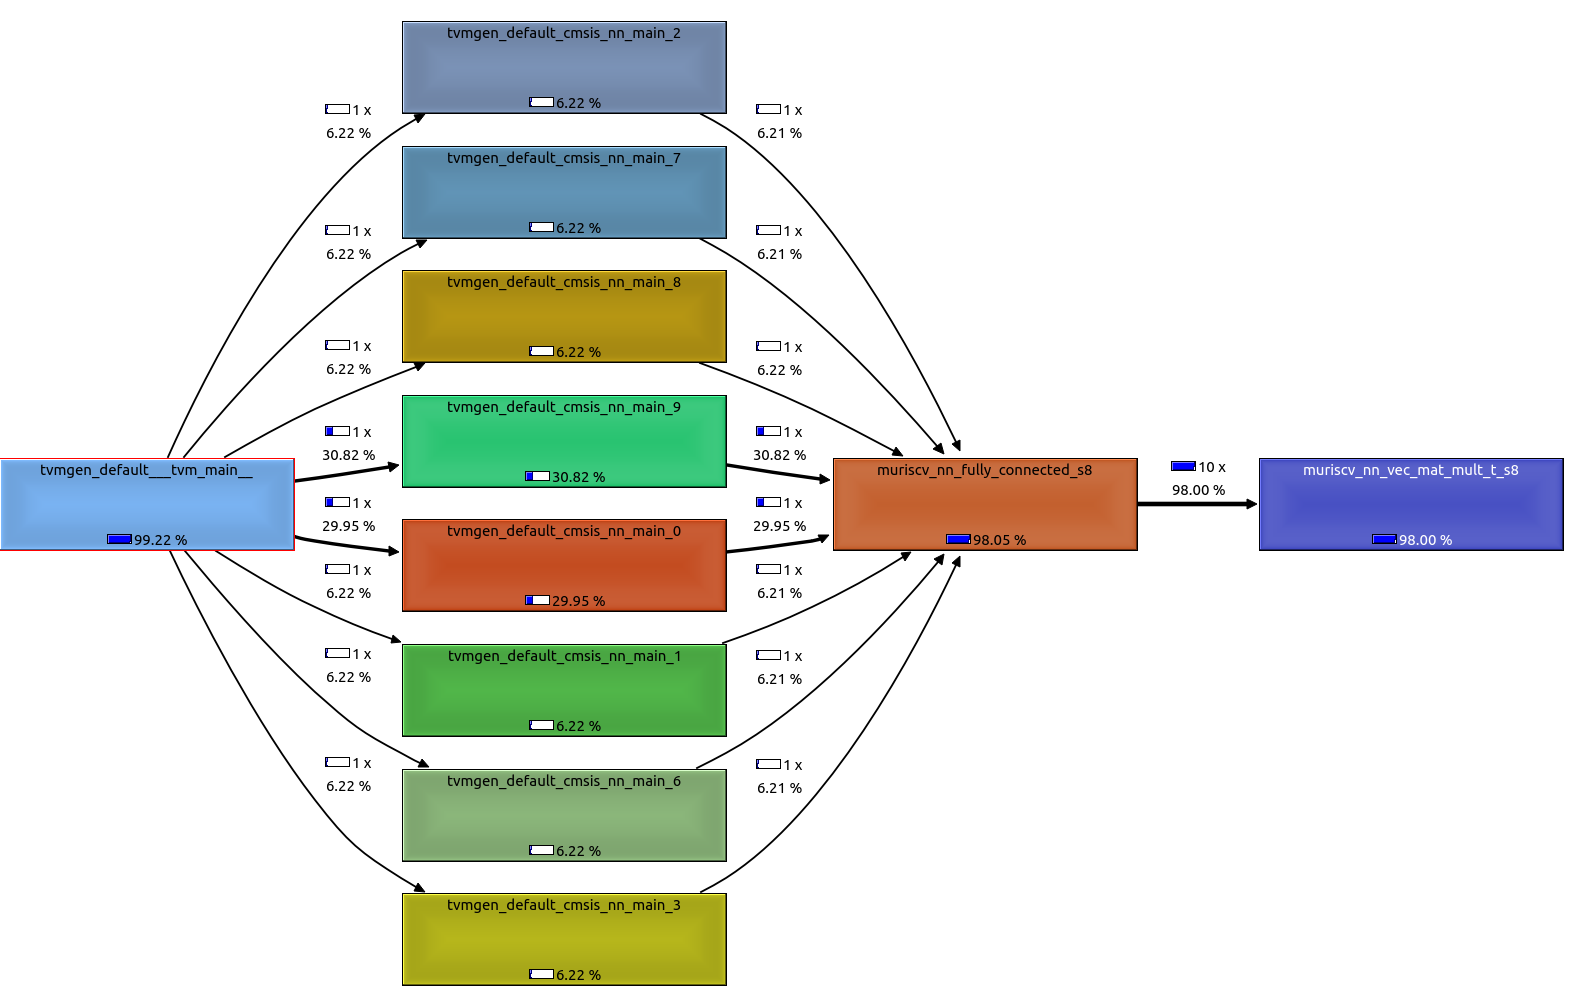
\includegraphics[width=.9\linewidth]{figures/evaluation_toycar_call_graph.png}
    \caption{Callgraph of toycar benchmark in kcachegrind}
    \label{fig:evaluation_toycar_call_graph}
\end{figure}

\begin{figure}[ht]
    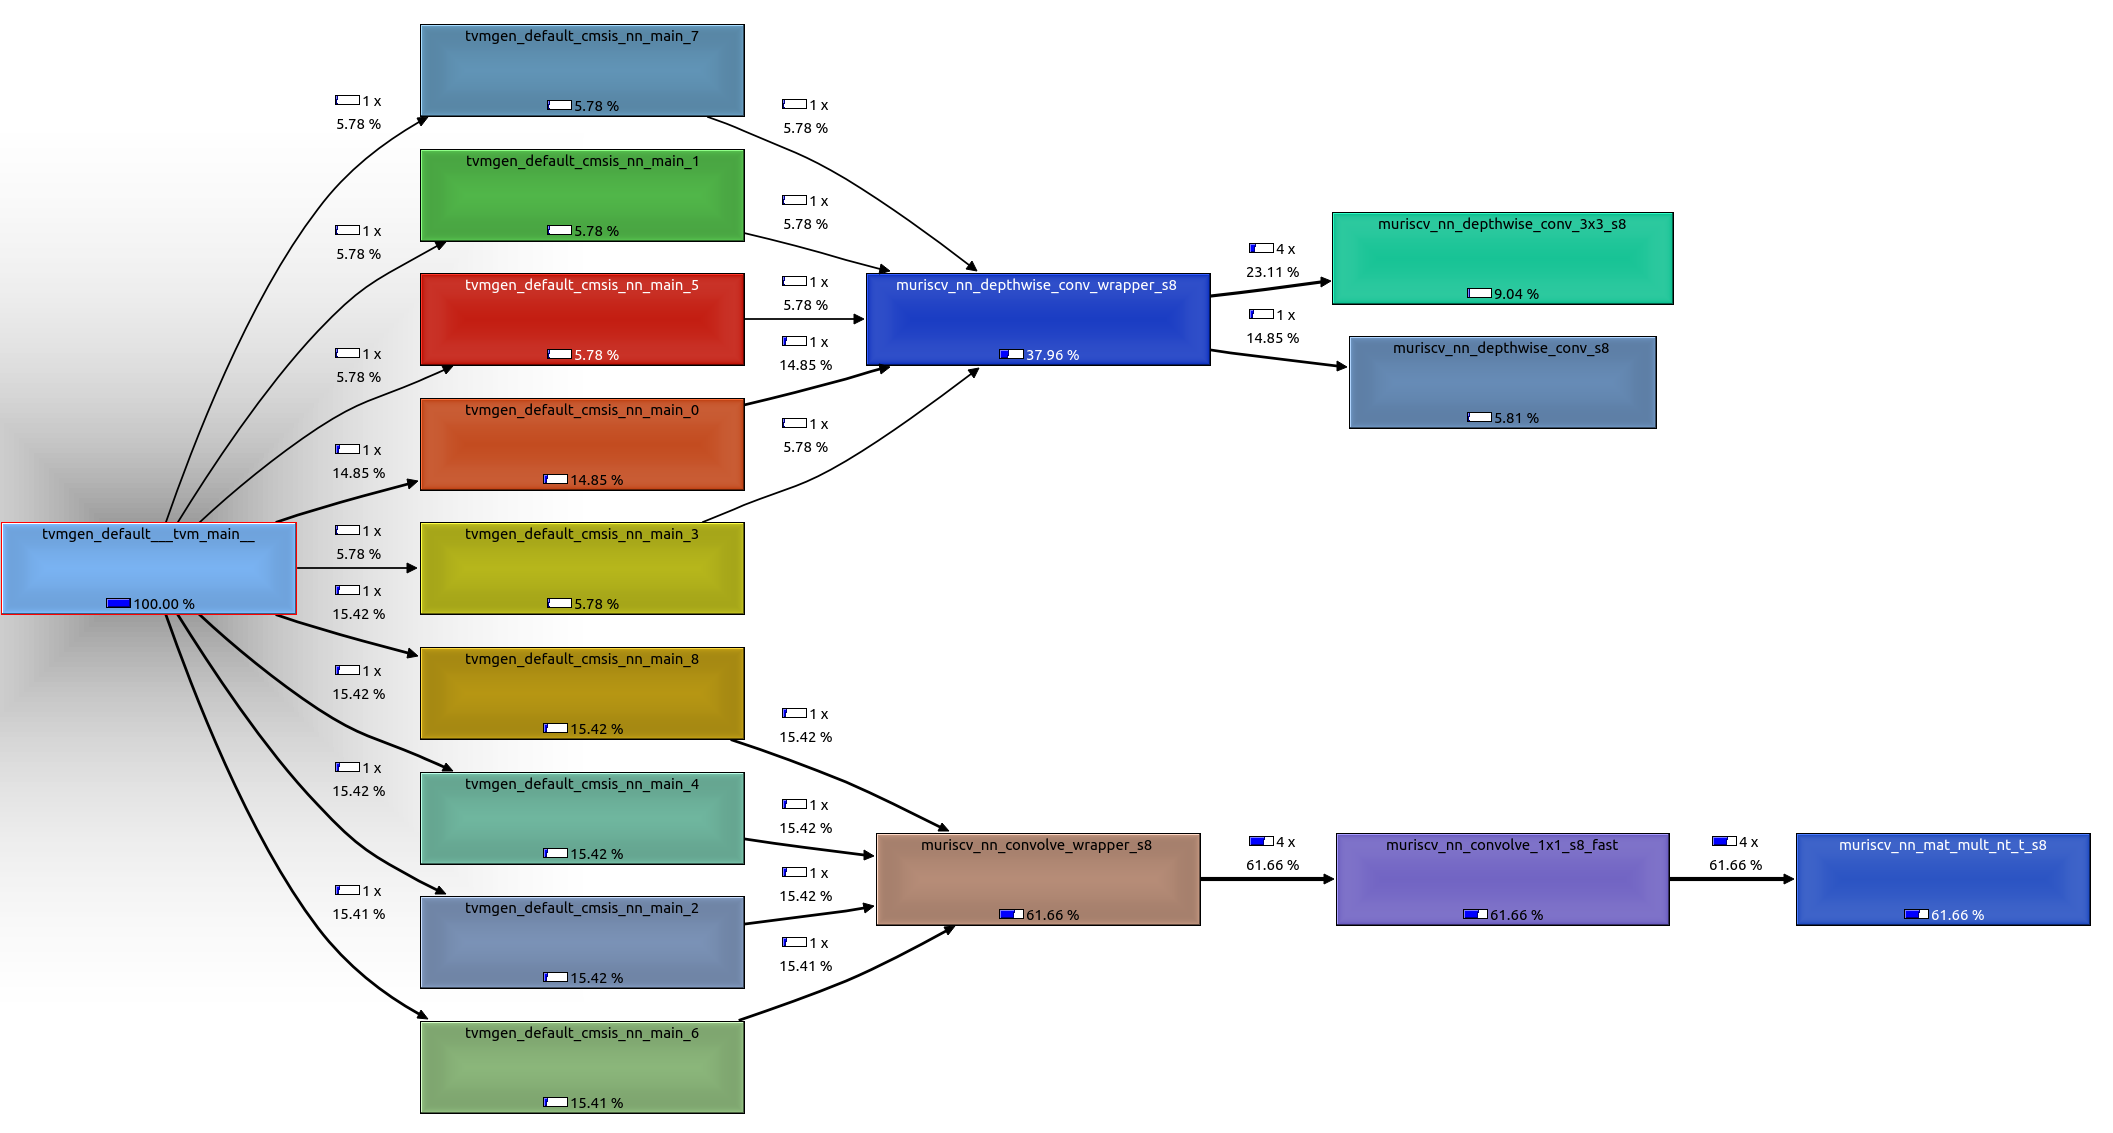
\includegraphics[width=\linewidth]{figures/evaluation_aww_call_graph.png}
    \caption{Callgraph of aww benchmark in kcachegrind}
    \label{fig:evaluation_aww_call_graph}
\end{figure}

\begin{figure}[ht]
    \centering
    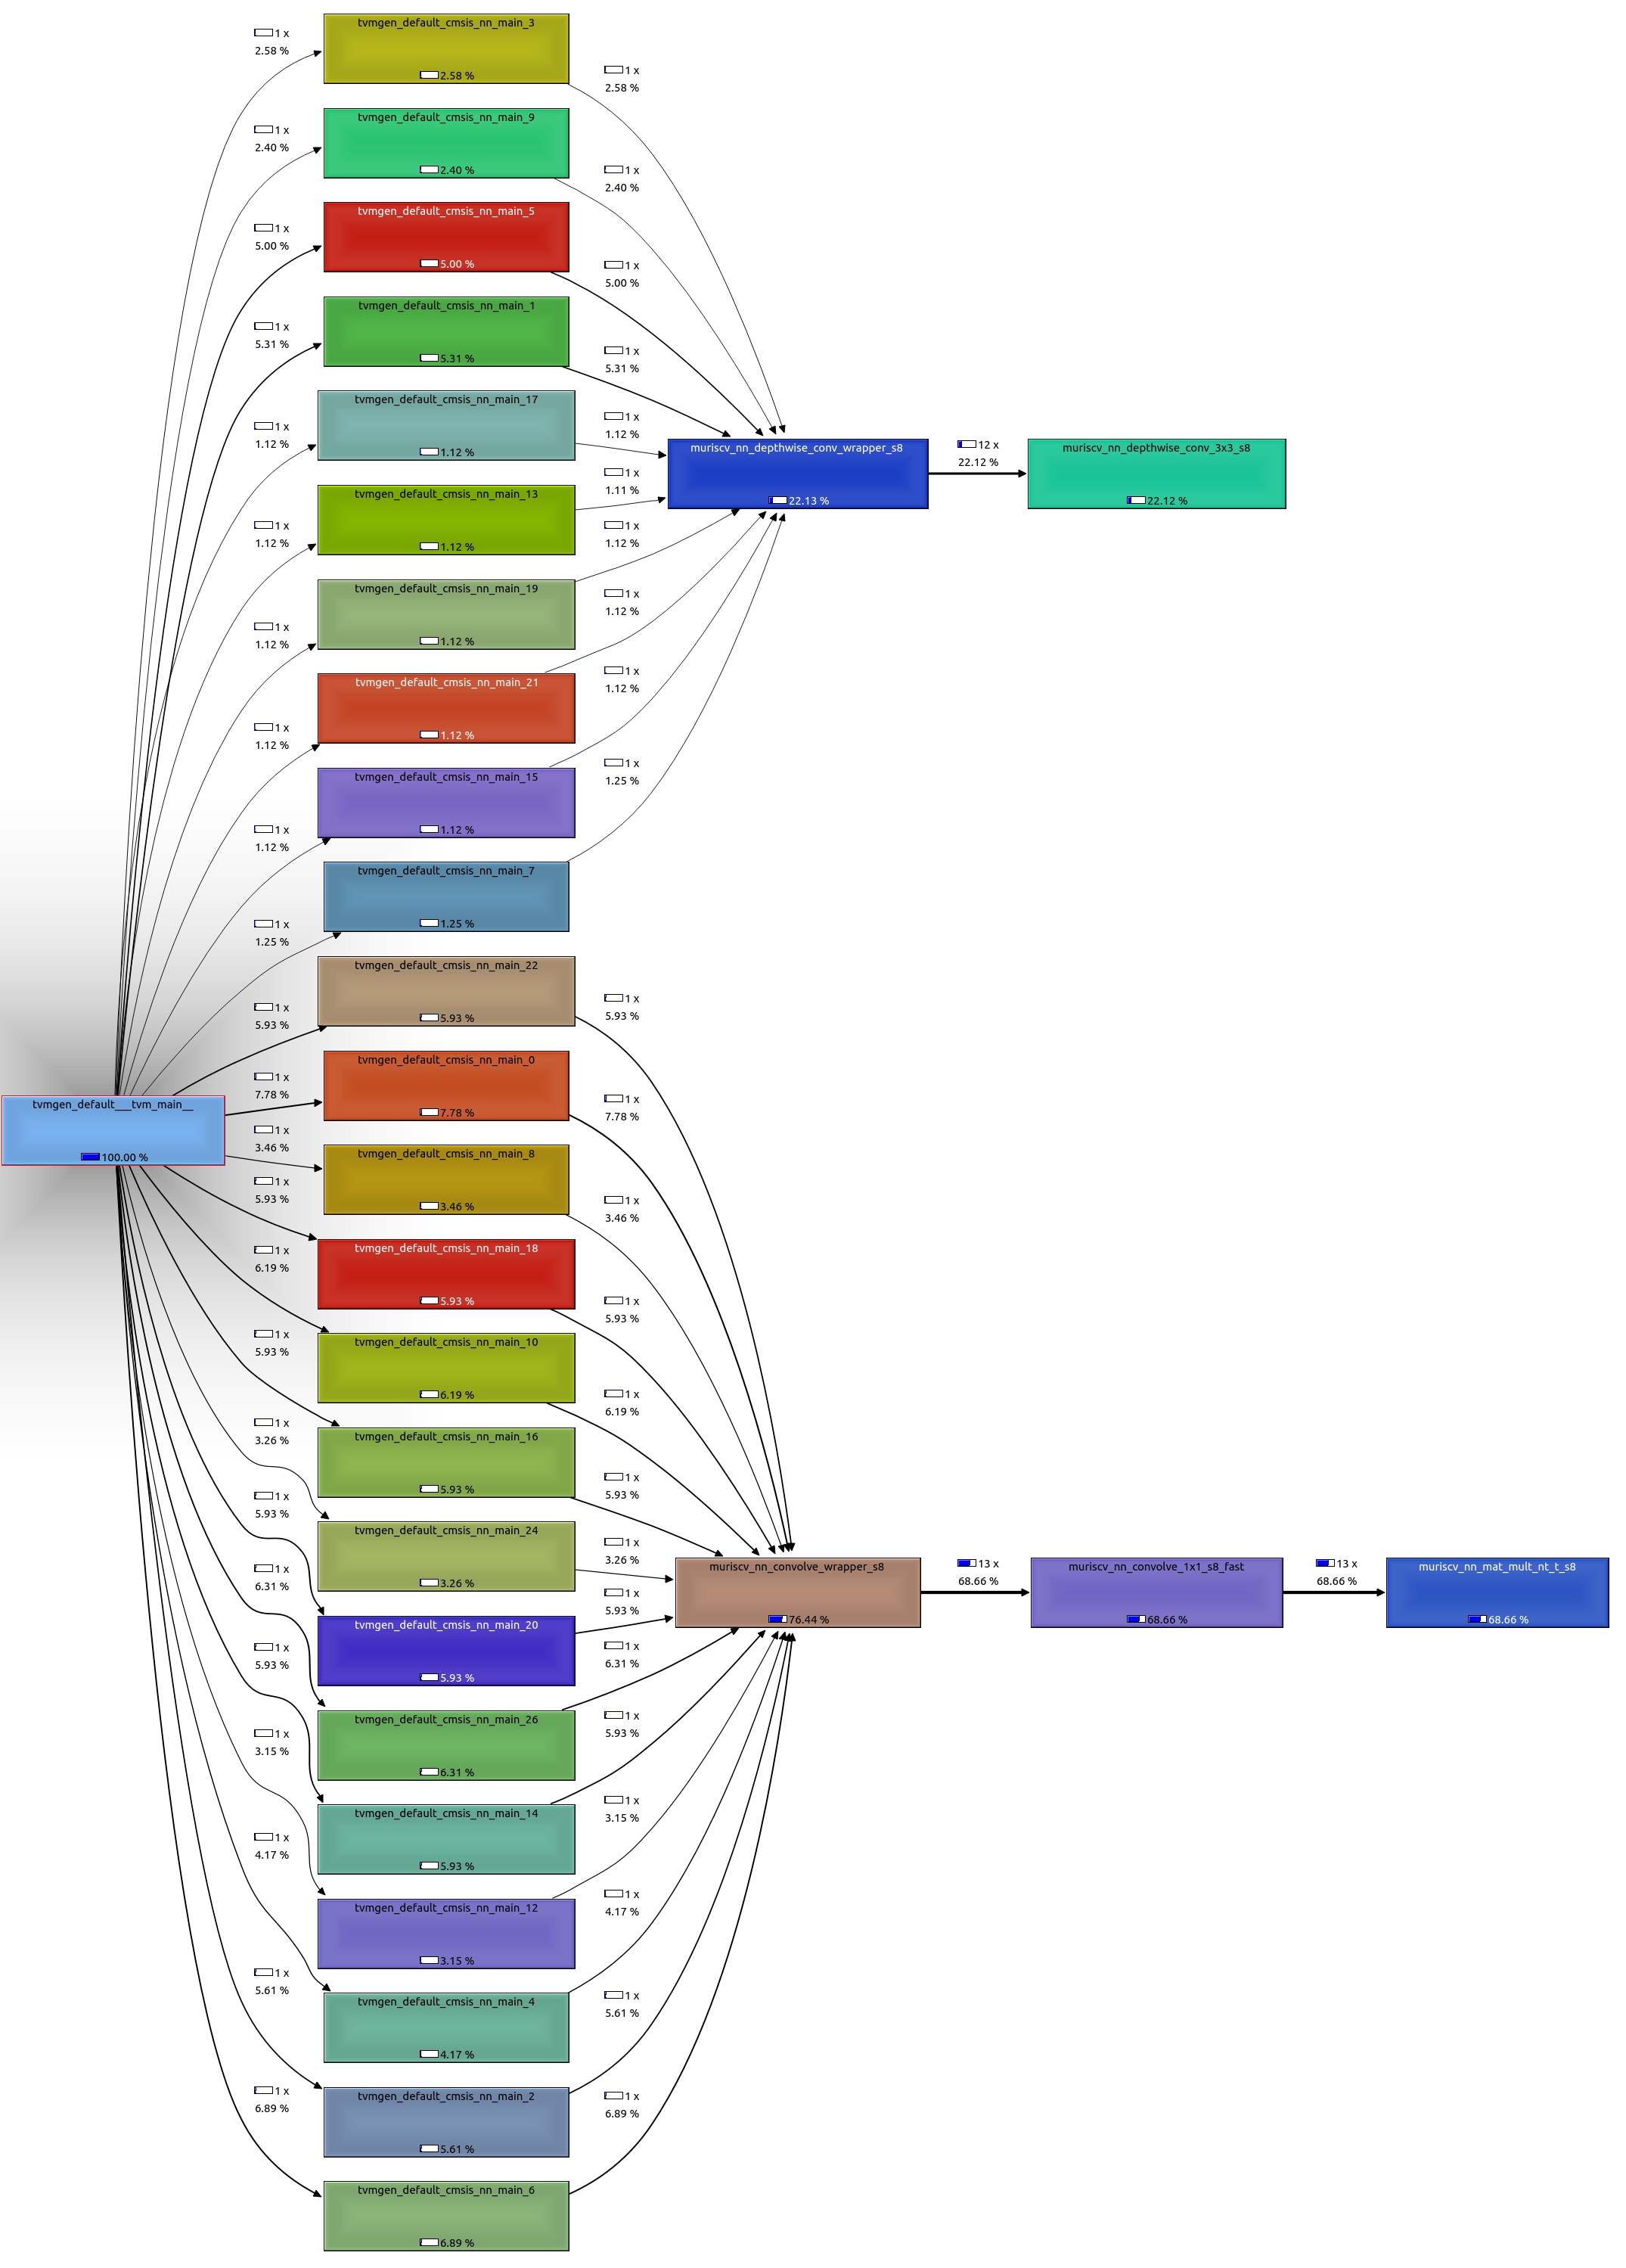
\includegraphics[width=.9\linewidth]{figures/evaluation_vww_call_graph.png}
    \caption{Callgraph of vww benchmark in kcachegrind}
    \label{fig:evaluation_vww_call_graph}
\end{figure}

\begin{figure}[ht]
    \centering
    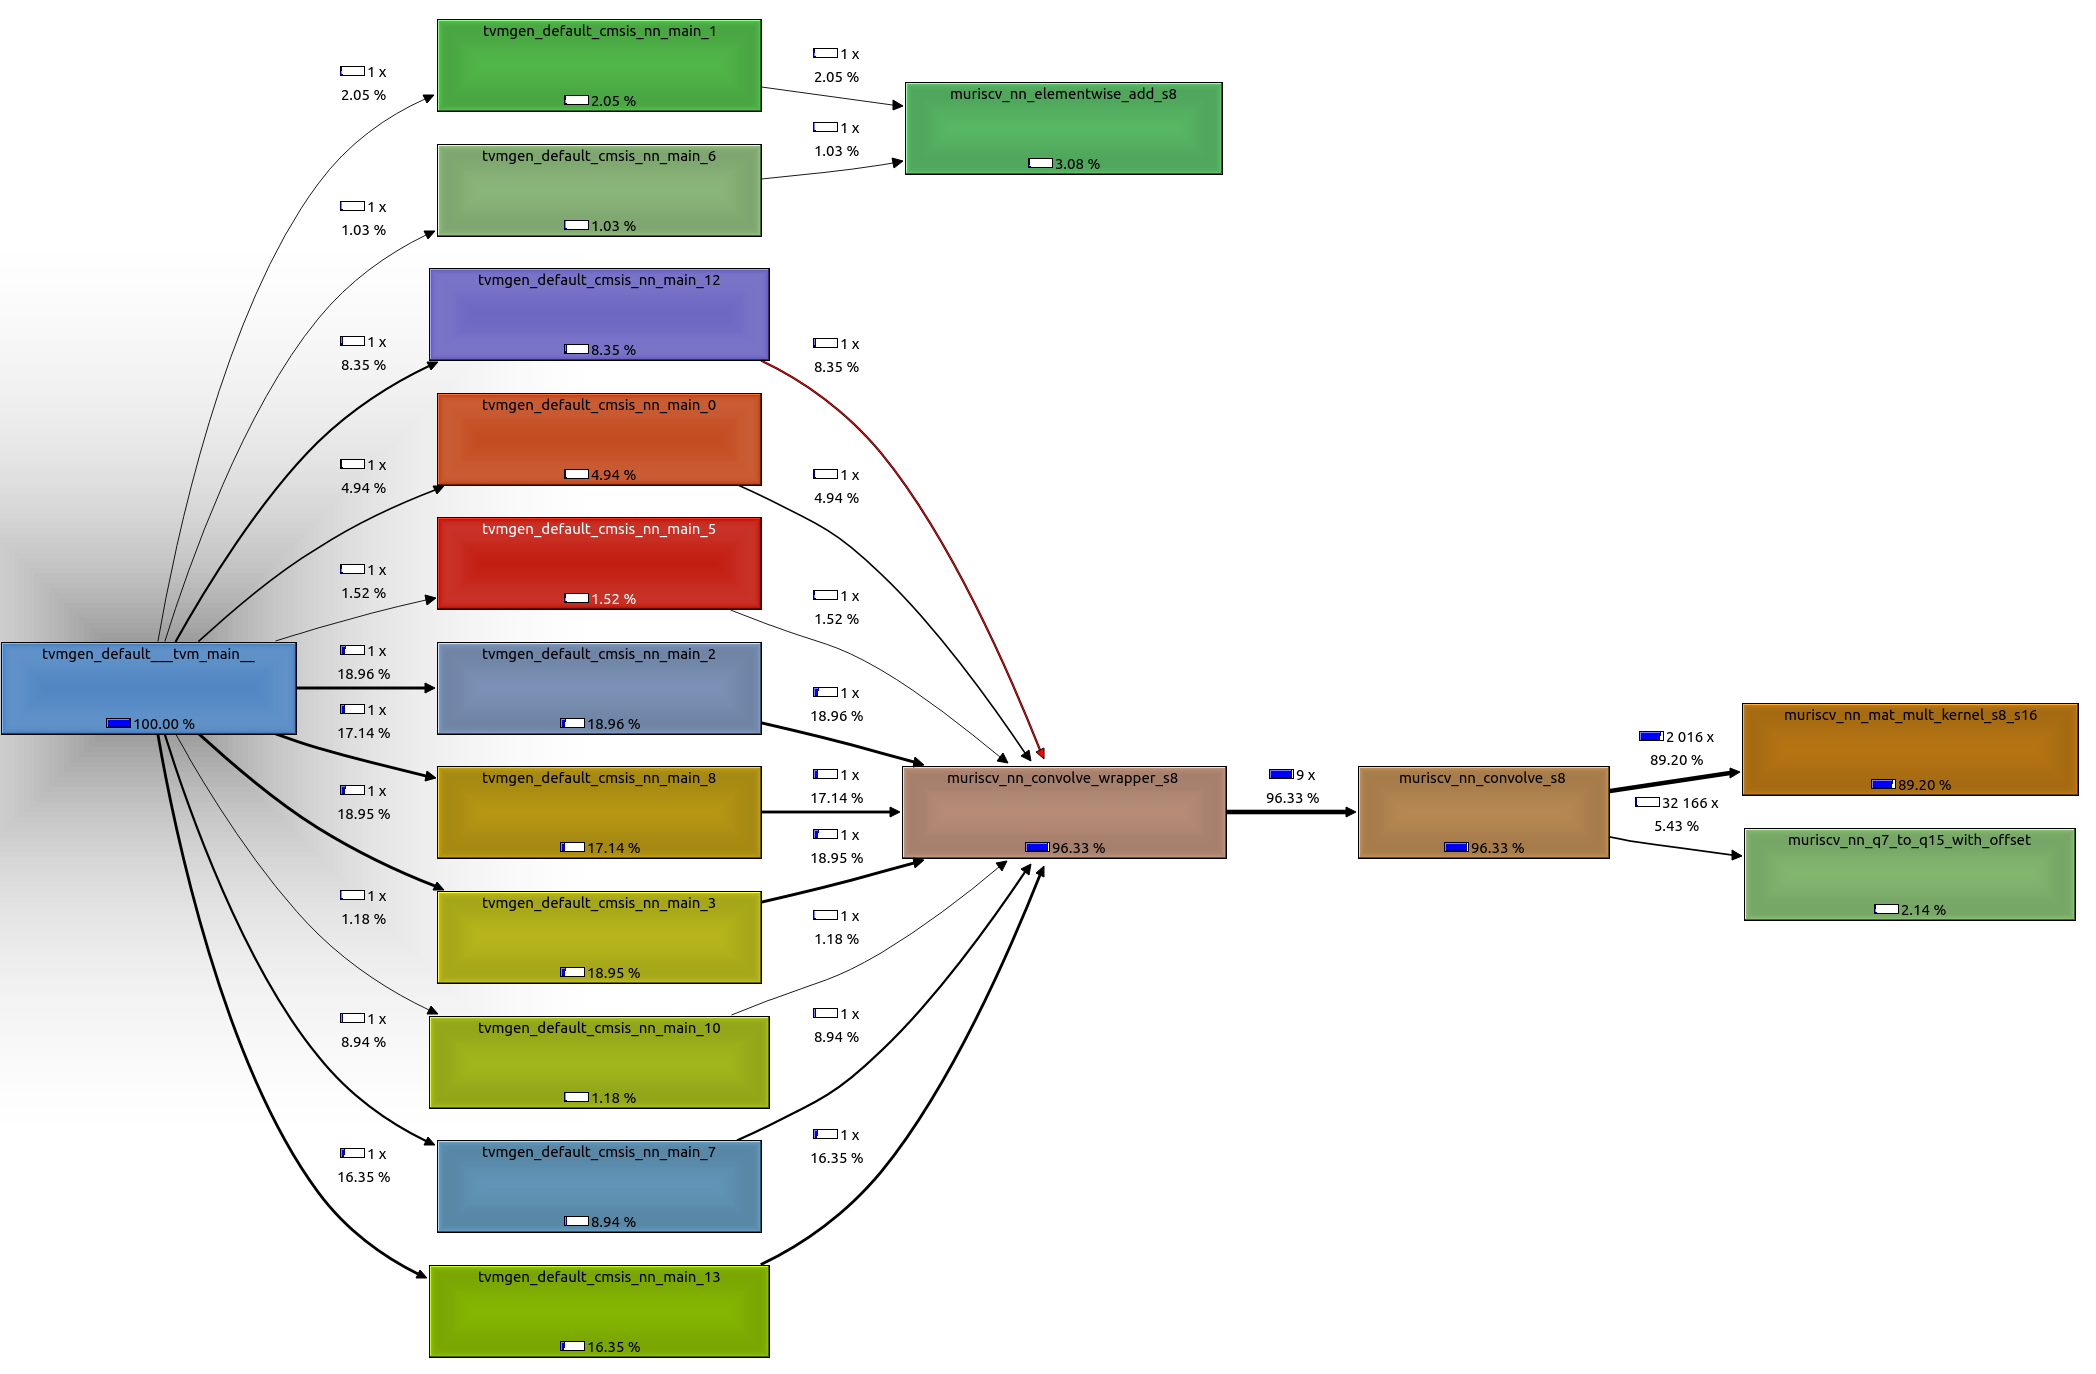
\includegraphics[width=.9\linewidth]{figures/evaluation_resnet_call_graph.png}
    \caption{Callgraph of resnet benchmark in kcachegrind}
    \label{fig:evaluation_resnet_call_graph}
\end{figure}


\microtypesetup{protrusion=false}

\addchap{Abbreviations}
\begin{acronym}
	\itemsep-.25\baselineskip
	\acro{TUM}[TUM]{Technical University of Munich}
    \acro{EDA}[EDA]{Electronic Design Automation}
    \acro{TinyML}[TinyML]{Tiny Machine Learning}
    \acro{ISA}[ISA]{Instruction set architecture}
    \acro{ETISS}[ETISS]{Extendable Instruction Set Simulator}
    \acro{SoC}[SoC]{Systems-on-chip}
    \acro{IR}[IR]{Intermediate Representation}
    \acro{PDLL}[PDLL]{PDL Language}
    \acro{JIT}[JIT]{just-in-time}
    \acro{ELF}[ELF]{Executable and Linkable Format}
    \acro{ASIP}[ASIP]{application-specific instruction set processor}
    % TODO: add acronyms
\end{acronym}

\listoffigures{}
\listoftables{}
\microtypesetup{protrusion=true}
\printbibliography{}

\end{document}
